\documentclass{article}
\usepackage{amsmath}
\usepackage{cite}
\usepackage{tikz}
\usepackage{bm}
\usepackage{tikz,tkz-tab}
\usepackage{amsfonts}%
\usepackage{amssymb}%
\usepackage{hyperref}
\usepackage{mathtools}
%\usepackage{subcaption}
\usepackage{color}
\usepackage{setspace}
\usepackage{empheq}
\usepackage{bbm, dsfont}
\usepackage{dsfont}
\usepackage{mathtools}
\usepackage{geometry}
\usepackage{enumitem} 
\usepackage[bottom]{footmisc}
\usetikzlibrary{arrows}
\usepackage{lscape}
\usepackage{tcolorbox}
\usepackage{caption}
%\usepackage{graphicx}
\usepackage{subfig}
\usetikzlibrary{shapes,snakes}
\renewcommand{\labelitemi}{$\bullet$}
\renewcommand{\labelitemii}{$\diamond$}


\newtheorem{definition}{Definition}

\usetikzlibrary{positioning}
\tikzset{main node/.style={circle,draw,minimum size=0.5cm,inner sep=0pt},
            }

%-------------------------------------------
\newtheorem{example}{Example}
\newtheorem{theorem}{Theorem}
\newtheorem{acknowledgement}[theorem]{Acknowledgement}
\newtheorem{algorithm}[theorem]{Algorithm}
\newtheorem{axiom}[theorem]{Axiom}
\newtheorem{case}[theorem]{Case}
\newtheorem{claim}{Claim}
\newtheorem{conclusion}[theorem]{Conclusion}
\newtheorem{condition}[theorem]{Condition}
\newtheorem{conjecture}[theorem]{Conjecture}
\newtheorem{corollary}{Corollary}
\newtheorem{criterion}[theorem]{Criterion}
\newtheorem{assumption}{Assumption}
\newtheorem{exercise}[theorem]{Exercise}
\newtheorem{lemma}{Lemma}
\newtheorem{observation}{Observation}
\newtheorem{notation}[theorem]{Notation}
\newtheorem{problem}[theorem]{Problem}
\newtheorem{proposition}{Proposition}
\newtheorem{remark}[theorem]{Remark}
\newtheorem{solution}[theorem]{Solution}
\newtheorem{summary}[theorem]{Summary}
\newenvironment{proof}[1][Proof]{\textbf{#1.} }{\ \rule{0.5em}{0.5em}}

\begin{document}

\title{ Hidden Opinions }

\author{Shaden  Shabayek\footnote{Universit\'{e} Paris1 Panth\'{e}on-Sorbonne, Paris School of Economics, 48 boulevard Jourdan 75014 Paris, France. Contact information: shaden.shabayek@sciencespo.fr.}}
%\date{July 30, 2020}
%\institute{Universit\'{e} Paris1 Panth\'{e}on Sorbonne \\ Paris School of Economics}

\maketitle

\begin{abstract}
This  paper widens the scope of analysis of opinion dynamic models by introducing a novel heuristic: individuals choose to express their opinion or hide it, as a function of their local popularity. Intuitively, individuals who hide their opinion could be interpreted as individuals who have a low popularity such that even if they speak-up (or $tweet$) they will not be heard.  Local popularity captures the idea that immediacy causes higher influence. Locally popular individuals express their opinion and can interact with like-minded or ideologically-opposed peers, namely expression entails debates and discussions.  In the presence of hidden opinions, I show that the interactions between locally popular individuals and the magnitude of their influence explains whether consensus or polarization prevails. The primary mechanism at play is that the influence structure allows for consensus of opinion locally but communication between ideologically opposed expressers lead to global disagreement. The main contribution of this paper is to provide a unifying theoretical framework to assess different long-run opinion patterns with a focus on the topology of the network.  I provide a measure of polarization and I run simulations to show the extent to which the topology of the network affects long-run opinion patterns.   
\end{abstract}
\medskip

\noindent {\sc \bf Keywords}: Naive learning, repulsive influence, opinion polarization. 

\medskip

\noindent {\sc \bf JEL Classification numbers}: D83, D91, Z1. 

%
%%\newpage
%%\tableofcontents
%
%\newpage

%\doublespacing
\onehalfspacing
\section{Introduction}

%By taking a simple walk on social media, one can effortlessly notice that not all voices are equal. Social media have become a new networked public sphere where influencers and politicians express themselves, interact among each other and supposedly with the rest of the population. In particular, opinion polarization is empirically well documented, yet its drivers remain unclear. So have social media connected or disconnected our societies? 
Are all people equal on social media or do popular voices dominate the conversation? My paper investigates this question by introducing a new heuristic to the study of opinion formation in social contexts. Namely I introduce an $expression$ $heuristic$, which assumes that individuals choose whether to express their opinion or hide it based on how popular they are within their social network. Individuals who hide their opinion can be interpreted as individuals who have a low popularity such that even if they speak-up they will not be heard or considered. One can think of an individual who has very few followers on Twitter. Alternatively, a second interpretation can be that hiding one's opinion is less costly than expressing it. The cost of expression can be the time spent arguing with more eloquent and persuasive peers or the cost of social isolation when one's opinion drifts from the average group viewpoint.
 
\bigskip

The $expression$ $heuristic$ departs from early models of opinion formation, such as French (1956)\cite{french}, Harary (1959)\cite{harary}, DeGroot (1971) \cite{degroot}. In these seminal models, individuals pool their opinions by taking the average of opinions expressed by all of their direct contacts at every period of interaction, irrespective of differences in levels of expertise or influence. When referring to this classic opinion updating rule, I say that individuals update their opinions \`{a} la DeGroot. In that framework, regardless of the specific topology of the network, as long as it is (strongly) connected and aperiodic, individuals reach consensus of opinion in the long-run. The present paper refines these contributions by relating the opinion updating rule to the topology of the network. Namely, I introduce two types of individuals with different opinion updating rules. In doing so, I provide a unifying framework to assess different long-run opinion patterns, such as consensus, polarization of opinion or total disagreement.

\bigskip

Formally, I develop a model where a set of individuals are connected through an undirected network and exchange opinions about a given issue over a large number of periods. Each individual is exogenously allocated an initial opinion in a bounded interval, which represents their initial stance or attitude concerning the issue to be discussed. The influence of each individual is summarized by a given real valued centrality measure.\footnote{In section \ref{simulations} I define a centrality measure, which I call $local$ $popularity$, and motivate its use.} As mentioned, there are two types of individuals: individuals who $hide$ and individuals $express$ their opinion. If the influence of an individual is below a given threshold (hereafter \textit{expression-threshold}), then they $hide$ their opinion and update their opinions \`{a} la DeGroot. Otherwise, individuals $express$ (hereafter $expresser$) and update their opinions according to a law of motion, which could incorporate either assimilation of opinions or distancing. At a given period, two directly connected expressers can either be like-minded or ideologically-opposed depending on the difference of their respective viewpoints. In particular, expressers only interact with peers who also choose to express. To be more precise, individuals who express undergo an attractive effect (positive influence or assimilation) when interacting at a given period with like-minded peers who also choose to express. But when they interact with expressing peers that are ideologically-opposed, they undergo a repulsive effect (negative influence or distancing) and push each other to the upper and lower bound of the opinion interval. Intuitively, expression allows for a debate or a discussion to take place. This discussion could lead to agreement or can escalate to conflict. 
%Two directly connected expressers are like-minded at a given period if the difference of their respective viewpoints is small enough, otherwise they are ideologically-opposed.
\bigskip
%The position of each individual in the network determines their local popularity, which is defined as the degree of an individual divided by the average degree of friends.

\bigskip

I provide a novel unifying framework that explains how different opinion patterns prevail in the long-run. In the presence of hidden opinions, the study of the interactions between locally $popular$ individuals who interact with like-minded or ideologically-opposed peers can explain whether consensus or polarization prevails. Since influence is stronger locally, clusters can form. But some members within a given cluster who are popular enough and interact with ideologically-opposed peers can fall into disagreement, which causes opinions to polarize across clusters. Expressers only pay attention to neighbors who also express, while consensual individuals who update their opinions \`{a} la DeGroot pay attention to all of their direct social contacts. This paper makes several contributions. First, I start by characterizing the opinions of expressers. Second I characterize the overall process of interpersonal influence with the two types of individuals and the two opinion updating rules. I show that opinions converge in the long-run. Third, I provide simulations to relate the specific topology of the network to the level of opinion polarization; defined as the variance in the long-run opinions. 

\bigskip

When an expresser has no neighbors who is also an expresser, this individual remains stubborn and their long-run opinion corresponds to their initial opinion. Furthermore, expressers can have neighbors who are locally popular and choose to express. For instance, consider three expressers $1$, $2$ and $3$. Individual $1$ has a direct link to $2$ and $2$ has a direct link to $3$, but $1$ and $3$ are not directly connected. Assume that all the remaining friends of those three individuals are not popular enough to express. The opinion update of individual $1$ depends on their opinion difference with individual $2$ and indirectly depends on the interaction between individual $2$ and $3$. Individuals $1$, $2$ and $3$ form a set of connected expressers. Namely, this set is defined as follows: all the elements of the set are nodes (individuals) who choose to express and any two nodes are connected by a path of expressers within this same set. 

With this definition in hand, proposition \ref{expressers} considers a group of individuals who belong to the same set of connected expressers and shows that, if each member of the set has only like-minded neighbors, then the long-run opinions of each member is exactly the average of the initial opinions of the members of this set. Each expresser of the group undergoes only the attractive effect. In particular, the group can have members who are ideologically-opposed that are not neighbors. But since they are not directly linked, they do not repulse each other to the upper and lower of the opinion interval and become extreme. Hence the whole group can reach consensus by gathering different viewpoints. This result sheds light on the design of media tools or the formation of discussion groups for initiatives related to participatory democracy.\footnote{For example, think of the Citizens' convention for climate (\textit{convention citoyenne pour le climat}) in France, where $150$ citizens were randomly selected to work in smaller groups on different propositions. } 

Proposition \ref{extreme} characterizes the long-run opinions within a connected set of expressers, when a pair of initially ideologically-opposed neighbors belong to the group. I show that, generically, the long-run opinions of the group of connected expressers reach the upper or lower bound of the opinion interval. That is, all the members of the connected group of expressers become extreme. One special case where  moderate opinions of expressers can survive in the long-run occurs when an expresser has like-minded neighbors. But they are indirectly connected to at least two ideologically-opposed expressing individuals. This case depicts a political left-right spectrum where parties on the far right and far left are ideologically-opposed and interact often together but between both parties, many moderate parties survive. 

\bigskip

Unlike linear models with assimilative influence, my model is non-linear; in the sense that the influence structure or the $hearing$ matrix\footnote{This matrix provides information on who listens to whom or who pays attention to whom and the magnitude of this attention.} can vary across periods in the presence of expressers who repulse or attract each other. Two expressers can initially be like-minded and influence each other positively. But in subsequent periods they can become ideologically-opposed and influence each other negatively, if one of them is repulsed by another expressing neighbor. Intuitively, this situation occurs when two individuals are somehow like-minded initially. But one of them starts adopting an extreme point of view in an unreasonable fashion under the influence of a third expressing peer, so her friend starts bringing to the table arguments which support the opposing view.  In other words, the weights in the hearing matrix can depend on the opinion itself, as in Hegselmann and Krause (2002)\cite{hegselmann}.

\bigskip
Lemma \ref{time} shows that the time or number of periods that two directly linked expressers take to repulse each other to the upper and lower bound of the opinion interval when they are ideologically-opposed, is smaller than the time they take to reach an agreement when they are like-minded. This motivates the study of the process of interpersonal influence with both types of individuals, starting from the time period by which repulsion opportunities in the course of a discussion are exhausted. I build a hearing matrix which accounts for both updating rules and show that opinions converge in the long-run. In particular, I show that the opinions of consensual individuals (who choose to $hide$) vanish in the long-run and remain hidden forever. Their long-run opinions simply become convex combinations of opinions of expressers to whom they are connected. Long-run consensus of opinions corresponds to an opinion vector such that the difference between any two opinions is small. Long-run bi-polarization of opinions corresponds to an opinion vector such that opinions belong to two groups of equal size: within each group opinions are close enough (below a threshold) and across both groups the opinion difference is large. 

Proposition \ref{consensus} provides necessary and sufficient conditions for consensus to prevail in the long-run. First, long-run consensus of opinions is obtained when there is a unique expresser. Second, consensus prevails when there exists multiple sets of connected expressers such that: $(i)$ within each set, all members have like-minded neighbors, $(ii)$ the average of initial opinions across two sets of connected expressers is close enough. Long-run opinions of consensual individuals depend on the long-run opinions of expressers to whom they are connected. Since those expressers all have similar viewpoints, consensual individuals adopt similar viewpoints when they take the average of opinions expressed within their social circle. The $type$ of consensus obtained will depend first on how many expressers there are in the society. Their number is directly related to the structure of the network. Second, it depends on the expressed opinions within the neighborhood of each expresser.  

Mapping back a long-run bi-polarized opinion vector to an exact set of  network structures and initial opinion distributions is tedious\footnote{Hegselmann and Krause (2002)\cite{hegselmann} have a non-linear model and they discuss this point extensively: \textit{though elementary, the model is nonlinear in that the structure of the model changes with the states of the model given by the opinions of the agents (see Section 2). Not only that helpful mathematical tools like Markov chains are no longer applicable, it turns out, moreover, that rigorous analytical results are difficult to obtain.}.}. Consensual individuals are influenced by expressers to whom they are linked directly and indirectly. Put simply, they receive influence of different magnitudes from many expressers depending on how far or close they are from those expressers in the network. That is, one needs to account for all the possible paths of different length connecting consensual individuals to expressers who may be ideologically-opposed. 

I provide compelling necessary conditions for long-run bi-polarization of opinions in lemma \ref{biplemma}. I show that if a long-run opinion vector is bi-polarized then necessarily, $(i)$ individuals who remain moderate in the long-run do not exist, $(ii)$ both extreme influence groups influence an equal share of the society. The first condition means that there does not exist individuals who receive an equal amount of influence from two ideologically-opposed extreme opinion groups. Those individuals occupy a very particular location in the network, because they are not locally popular enough to express and they are equally influenced by two ideologically-opposed groups of expressers. Those individuals could be interpreted as neutral TV hosts, or non-biased journalists or intermediaries in general.
%\footnote{The Matlab code for the simulations can be found on the GitHub repository \href{https://github.com/shadenshabayek/Hidden-Opinions/}{\color{blue}shadenshabayek/Hidden-Opinions}.}  

{\bf Simulations.} I explore the model through simulations.\footnote{The Matlab code can be found in the following repository \href{https://github.com/shadenshabayek/Hidden-Opinions}{https://github.com/shadenshabayek/Hidden-Opinions}. } The objective is to relate the topology of the network to the long-run opinion patterns. Polarization of long-run opinions is measured by taking the variance of final opinions. I generate initial opinions uniformly at random in a bounded interval and study the evolution of opinions of a large set of individuals in scale-free networks. The degree distribution within scale-free networks follows a power law. Due to this inequality in the degree distribution, expressers and consensual individuals co-exist. %The objective of the simulations is to make obvious the impact of the interaction structure - location in the network and initial opinion - of expressers on the long-run opinion pattern of the whole group of individuals. Scale-free networks are meant to model Twitter-like networks where there are $stars$ or $influencers$ with many followers and where stars have the opportunity to interact together. First, I provide two examples where I show how the density of connections among expressers affects the average level of polarization, for two specific network topologies of scale-free networks. More interaction between expressers leads in average to higher levels of polarization. Second, I provide aggregate statistics on different network topologies of scale-free networks by varying the number of initial hubs and the number of connections a newly added node has. Doing so allows me to relate different scale-free network topologies to the average level of polarization. Those statistics are divided into two groups: $(i)$ (inter-related) measures of degree inequality $(ii)$ and measures of connectivity. 
In particular, this exercise shows that average polarization level can be relatively low even if expressers are densely connected among each other. This happens precisely for network topologies where consensual individuals are connected to many influence sources.

\bigskip

{\bf Related literature.} The study of opinion dynamics is a multi-disciplinary topic. Different fields such as economics (learning in networks, for surveys see Golub and Sadler (2017)\cite{golubsadler} and Acemoglu and Ozdaglar (2011)\cite{acemoglu}), sociology (the community cleavage problem, see Flache et al. (2017)\cite{flachesurvey2017} or Friedkin (2015)\cite{friedkin2015}),  statistical physics and computer science (community detection, Malliaros and Vazirgiannis (2013)\cite{malliaros} survey the literature) have tackled this problem from different angles. 

This paper is closely related to a strand of the literature on Naive Learning which introduces $stubborn$ agents or agents that remain attached to their initial opinion to a certain extent, in order to model disagreement (See Friedkin and Johnsen (1990)\cite{friedkin} and Friedkin(2015)\cite{friedkin2015}, Acemoglu et al (2013)\cite{acemoglu2013}). Two papers that are closest to mine are Yildiz et al. (2013)\cite{yildiz2013} and Sadler (2019)\cite{sadler}. Both papers introduce $stubborn$ agents in a voter model set-up where opinions are discrete and can take only two discrete real values either $a$ or $b$. Players can be either stubborn, that is they never update their opinion, or they can update \`{a} la Degroot. Nevertheless, the stubbornness of a player is independent of their network position. Hence a stubborn player who is nor locally nor globally central can have a great impact on the long-run opinions of all individuals in the network. With that respect, I extend this approach by relating the impact a stubborn player can have on others' long-run opinions, to their popularity.  %My paper extends these two papers by considering stubborn agents as a special case that can occur when an expresser does not update their opinion because they have no expressing neighbors. Furthermore, I allow for opinions to take continuous values in the bounded interval $[a,b]$. Hence, my model can also explain the survival of moderate opinions (not at the upper bound $b$ or lower bound $a$) in the long-run. %% Here point is more in their model a stubborn agent with no particular influence or network position can attract all opinions... this cannot happen in my model 

My paper also fits in the family of bounded confidence models (See Hegselmann and Krauss (2002)\cite{hegselmann}, Jager and Amblard (2005)\cite{jager}). The key ingredient of those models is to consider the difference between the opinions of individuals when opinion updating is taking place. In particular, Hegselmann and Krauss (2002)\cite{hegselmann} consider a model where agents update their opinions by taking an average over the opinions of neighbors whose opinion difference falls within a confidence interval. When neighbors opinions fall outside the confidence interval they are ignored. I extend this literature by introducing an opinion updating rule which treats the opinions of neighbors differently, depending on whether the opinions of neighbors fall within or outside the confidence interval. 

Furthermore my paper is related to an active line of research about disagreement in social contexts and oppositional identity. Both literatures use different methodologies (dyadic interaction between agents versus interaction with a proportion of agents) but address very similar questions. 
Melguizo (2018)\cite{melguizo} studies persistent disagreement. She allows interactions and attitudes to co-evolve, hence departing from the time independent weights used in averaging neighbors' opinions in models \`{a} la DeGroot. The key ingredient used is to assume that each individual has several attributes. Relations with other individuals sharing similar attributes become more intense, while relationships with dissimilar others deteriorate. Furthermore, disagreement can modeled by introducing repulsive or negative influence when an individual interacts with dissimilar others or by modeling individuals who are similarity biased (See Flache et al. (2017)\cite{flachesurvey2017} for a survey). As for oppositional identity, Bisin et al. (2016)\cite{bisinzenou} provide a model which incorporates cultural conformity and cultural distinction, in the context of mariage choice within the same ethnic group or outside. Individuals select their optimal choice by considering the psychological cost of interacting with the proportion of dissimilar others. 

% both cultural conformity and cultural distinction. Cultural conformity and cultural distinction provide distinct empirical implications on the way neigh- borhood segregation interacts with the process of ethnic integration. When cultural conformity is the main motivational process of identity formation, we expect neighborhood segregation to act as a complement to ethnic assimilation. On the contrary, when cultural distinction is at work, neighborhood segregation might substitute for ethnic assimilation

%Patacchini and Zenou (2016)\cite{patacchinizenou} \\
%Toni and Guinjoan (2018)\cite{rodon} \\
%Cerreia-Vioglio et al. (2020) \cite{cerreia} \\

%My paper is related to the active line of research that models disagreement in social contexts (See Flache et al. (2017)\cite{flachesurvey2017} for a survey). Disagreement is modeled either by introducing repulsive or negative influence when an individual interacts with dissimilar others or by modeling individuals who only take into account opinions of others when they are close enough. Nevertheless, the role played by the specific topology of the network is not yet at the center stage of this literature. The results are often based on random pair interaction or a specific topology is given by assumption. Deffuant et al. (2000)\cite{deffuant} and Grow (2017)\cite{grow} consider individuals who are randomly paired and engage in dyadic interaction.   (e.g. Deffuant et al. (2000)\cite{deffuant}, Grow (2017)\cite{grow}, Krueger et al. (2017)\cite{krueger}, Axelrod (1997)\cite{axelrod}). Krueger et al. (2017)\cite{krueger} in a framework of a voter model assume that the social network has a double-clique topology consisting of two complete graphs connected by some cross lins with each other. Axelrod (1997)\cite{axelrod} in his seminal paper assumes that individuals are distributed over a $10$ by $10$ grid. 

Finally, explaining polarization has been tackled by a handful of recent papers, yet there is no consensus in the literature about its main drivers. Bolletta and Pin (2019)\cite{bolletta} introduce a network formation model and argue that under certain conditions when agents optimally choose their links, the network can become disconnected and consensus of opinions cannot be reached. Banisch and Olbrich (2019)\cite{banisch_olbrich} explain the emergence of polarization by introducing reinforcement learning, where agents optimally adopt one viewpoint when they get positive feedback from peers. But their focus is not on the network structure itself and how it could be one of the drivers, in particular they fix a random geometric network to account for the structure of interactions. 
\bigskip

{\bf Outline.} The remainder of the paper is organized as follows. Section \ref{socialpsychology} reviews relevant literatures in social psychology that lay the ground for the main behavioral assumptions of my model. In section \ref{themodel}, I present the model and I characterize the overall process of interpersonal influence in section \ref{eq}. In section \ref{simulations}, through simulations I relate the topology of networks to long-run opinion patters. Section \ref{conclusion} concludes. 

%%%%%%%%%%%%%%%%%%%%%%%%%%%%%%%%%%
\section{Related work in social psychology: Hidden Profiles} \label{socialpsychology}
%The two main novel ingredients of the model are the expression heuristic and the local popularity measure. The former ingredient is grounded in a well known literature in social psychology called Hidden Profiles\footnote{See the survey \textit{Hidden Profiles: a brief history} by Stasser and Titus (2003)\cite{stasser2003}} and the latter is borrowed from the Dynamic Impact Social Theory. In what follows I briefly review both literatures. 

%\subsection{Hidden Profiles}
Stasser and Titus (1985)\cite{stasser} document how individuals in social contexts, do not always share their own opinion or the information they hold. The starting point of their research is to challenge the common belief that a group of individuals should be able to take a better decision than each individual on their own by pooling the members' knowledge and expertise. Namely, group discussion or communication is believed to have a corrective function because members can each have incomplete information but together they can gather the different pieces of the puzzle. The authors ran an experiment in which they simulate a political set-up where a group has to elect one of three candidates: $Best$, $Okay$ and $Ohum$. In a first protocol, they distributed a different subset of desirable traits of $Best$ and a different subset of $Okay$'s undesirable traits over the members of the group, such that from each one's individual perspective $Okay$ appeared more positive than $Best$. Before discussion $Best$ received $25\%$ of endorsement. Since the whole group had complete (but dispersed) information about $Best$ they could exchange it and come to the conclusion that $Best$ was actually the best candidate. Yet after group discussion, surprisingly the percentage of endorsement for $Best$ remained at $24\%$. This finding suggests that unique information held by some members of the group about candidates were not being shared. In a later study, Stasser, Taylor and Hanna (1989)\cite{stasser89} showed that unique pieces of information are less likely to be mentioned during group discussion.  %\textit{Each member received a different subset of Best's desirable traits and a different subset of Okay's undesirable traits. As a result, from the perspective of any one member, Okay appeared to have more positive and fewer negative traits than did Best. Nonetheless, the group as a whole had complete information and, by exchanging their unique information, could have ascertained that Best was better than Okay.}
One explanation is that social status, expertise or popularity can be a driver for expression of opinion. In fact, Larson et al. (1996)\cite{larson} suggest that repeating a unique piece of information, leading to the formation of group opinion during a discussion, is more likely by higher status members (experts, leaders, etc.) rather than lower status members. They ran an experiment with residents, interns and 3rd-year medical students and they show that residents were more likely to repeat (unique) information when compared to interns and students.

Using the findings of the above literature, I introduce an expression heuristic to a dynamic opinion formation model. An individual chooses to express her opinion or hide it based on a  popularity measure that is meant to capture different hierarchical and expertise levels. 



\section{The model} \label{themodel}

\subsection{Set-up} \label{setup}
A group of individuals $N=\{1, \ldots , n\}$ is embedded in a connected and symmetric network $G$ of interpersonal relationships, with typical entries $g_{ij} = g_{ji}  \in \{ 0,1\}$. Each node represents an individual. The set of friends of individual $i \in N$ is denoted by $N_i = \{j \in N : g_{ij}=1 \}$ and $d_i = |N_i|$ is the cardinality of $N_i$. For all $i \in N$, I assume that $g_{ii} =1$. A chain of friends of friends of length $l$ between two individuals $i \neq j \in N$, hereafter called  $path$,  is defined as follows: there exists a sequence of distinct individuals $i=k_0, k_1, \ldots, k_l = j \in N$ such that $g_{ik_1} \times g_{k_1 k_2} \times \ldots \times g_{k_l j} > 0$. The influence of each individual in the network $G$, is measured by a given real valued centrality measure which depends on the network topology, denoted by $\delta_i (G)$ for individual $i \in N$. 


\subsection{Expression heuristic}

Each individual $i \in N$ is endowed with an exogenous initial opinion $\alpha_{i,0} \in [-1,1]$ which represents their stance about a given issue.\footnote{Can model the issue as $\theta \in [-1,1]$ and make the network depend on it.} Individuals exchange opinions about the issue over $t \geq 0$ periods and they can be like-minded or ideologically-opposed. 

\begin{definition} At period $t \geq 0$, for $\tau \in (0,1)$, two individuals $ i \neq j \in N$ are :  \begin{itemize} \item[(i)]  $like$-$minded$, whenever $|\alpha_{i,t} - \alpha_{j,t}| < \tau$, \item[(ii)] \textit{ideologically-opposed}, whenever $|\alpha_{i,t} - \alpha_{j,t}| \geq \tau$. \end{itemize} \label{definition_likeminded} 
\end{definition}

At period $t$, each individual $i \in N$ observes the opinions in their neighborhood, denoted by ${\alpha}_{j,t} \in [-1,1]$ for all $j \in N_i$. At period $t+1$, each individual updates their opinion according to a rule which depends on their centrality: 

\begin{equation*} 
	\begin{cases}
		 \text{ Hide (rule 1) } & \text{ if } \delta_i (G) < \delta^{*} (G) \\
		\text{ Express (rule 2) } & \text{ if } \delta_i (G) \geq \delta^{*} (G),
	\end{cases}
\end{equation*} 
\bigskip

\noindent where $\delta^{*}$ denotes an exogenous threshold. In the remainder of the paper, the set of individuals who express will be labelled $E=\{ i \in N, \text{ s.t. } \delta_i (G) \geq \delta^{*} (G) \}$. \\

{\noindent \bf Hide (rule 1 or DeGroot)}: when an individual hides their opinion, they update their opinion by taking the average of opinions expressed within their social circle at the previous period: 
\begin{equation} 
\alpha_{i,t} = \overline{\alpha}_{i,t-1} = \frac{1}{d_i}  \sum_{j  \in N} g_{ji} {\alpha}_{j,t-1}. \label{average}
\end{equation}
  
{\noindent \bf Express (rule 2)}: when an individual expresses, the opinion updating process depends on: $(i)$ the opinions of neighbors, who also express and $(ii)$ whether two neighbors are like-minded or ideologically opposed (see Definition \ref{definition_likeminded}). More precisely, expression allows for a debate and the opinion updating process of expressers follows a law of motion which allows for agreement and disagreement. It incorporates an attractive (agreement) and a repulsive (disagreement) effect among direct neighbors who express their opinions. For all $ i \in E$ and {\color{red}$\mu \in (0,1/2)$}: 
%Law of motion
 \begin{equation}
 \alpha_{i,{t}} =  \alpha_{i,{t-1}} +  \mu \big( \sum_{j \in \underline{N}_{i,t-1}}   (  \alpha_{j,t-1} - \alpha_{i,t-1} ) - \sum_{j \in \overline{N}_{i,t-1}} ( \alpha_{j,t-1} - \alpha_{i,t-1} ) \big)  \text{ s.t. } \alpha_{i,t} \in [-1,1],
 \label{lawofmotion}
 \end{equation}

Where $\underline{N}_{i,t} =\{ j \in N_i \cap E, |\alpha_{i,t} - \alpha_{j,t}| < \tau\}$ and $\overline{N}_{i,t} =\{ j \in N_i \cap E, |\alpha_{i,t} - \alpha_{j,t}| \geq \tau\}$. 

\bigskip

\noindent Notice that, expressing neighbors receive influence from their own expressing neighbors (if any). Hence, an initially like-minded expressing neighbor of individual $i$ can become in subsequent periods ideologically-opposed, if their opinion difference with $i$ becomes larger than $\tau$.
\smallskip

 %Similarly, the set of individuals who hide their opinions will be labelled $C=\{ i \in N, \text{ s.t. } \delta_i < \delta^{*} \}$.   


\begin{example} Consider a network $G$ with only two connected individuals $1$ and $2$ who choose to express. Suppose that $\tau=0.5$ and initial opinions are  $\alpha_{1,0}=-0.7$ and $\alpha_{2,0}=0.7$. In period $t=1$, $\alpha_{1,1} = \alpha_{1,0} + \mu_{} ( \alpha_{1,0} - \alpha_{2,0}) =  -0.7 (1 + \mu) - \mu 0.7 < \alpha_{1,0} = -0.7 $ and  $\alpha_{2,1} = \alpha_{2,0} + \mu_{} ( \alpha_{2,0} - \alpha_{1,0}) = 0.7 (1+\mu) + \mu 0.7 > \alpha_{2,0} =0.7$. The updated opinion of individual $1$ becomes more negative or pushed-down towards $-1$, while the updated opinion of individual $2$ more positive or pushed-up towards $1$. Individuals $1$ and $2$ repulse each other. 
\end{example} 

 %Equivalently, the number of elements in the sets $\overline{N}_{i,t}$ and $\underline{N}_{i,t}$ of like-minded or ideologically-opposed expressing neighbors of individual $i \in N$ at a given period $t \geq 1$ can vary across two periods.  For instance, at period $t-1\geq 0 $ individual $j$ can belong to $\underline{N}_{i,t-1}$ but at period $t$ they can move to the set $\overline{N}_{i,t}$ as they can be influenced when updating her opinion by other expressing neighbors.   




%%%%%%%%%%%%%%%%%%%%%%%%%%%%%%%%%%%%%%
\section{Opinion Dynamics} \label{eq}

Given the above model, I am interested in studying the long-run opinions, for a network structure $G$ and a vector of initial opinions $\alpha_0$. Then I characterize in section \ref{convergence} the overall dynamics of opinions and show that long-run opinions always converge.  

\subsection{Long-run opinions of expressers}
\label{LRexpressers}

%%%
Individuals who choose to express update their opinions at each time period according to the law of motion \eqref{lawofmotion}. Consequently, their opinion update will directly depend on the opinions of neighbors who choose to $express$ (if any). The opinions of the latter will depend on the opinions of their own neighbors (if any) who choose to $express$ and so on. Recall that $E$ is the set of individuals who choose to express because their local popularity is higher than the expression threshold $\delta^{*}$. In order to account for the indirect effect of the opinions of expressers on other individuals who also express, I give a formal definition of a connected set of expressers. 

\begin{definition}[Connected set of expressers]
Let $G$ be a given network structure and let $\mathcal{E}$ be a set of individuals such that $(i)$ $\forall i \in \mathcal{E}$, $\delta_i \geq \delta^{*}$, $(ii)$  $\mathcal{E} \subseteq E$  and $(iii)$ any pair of individuals $i \neq j \in \mathcal{E} \subseteq E$ are connected in network $G$ by a path of length $l_{ij}$ of expressers belonging to the set $\mathcal{E}$,  that is $\exists g_{ik_1} \times g_{k_1 k_2} \ldots \times g_{k_l j} >0$ for $k_1, \ldots k_l \in \mathcal{E} \subseteq E$. When expressers $k_1, \ldots k_l \in \mathcal{E} \subseteq E$ all have like-minded neighbors, I say that individual $i$ is linked to individual $j$ through a path of like-minded expressers and denote it by $l_{ij}^{+}$. 
\label{connectedexpressers}
\end{definition}



In a given network there could be multiple connected sets of expressers $\mathcal{E}_1, \ldots, \mathcal{E}_k$ such that $E= \bigcup_{i=1}^{k} \mathcal{E}_i$. Those sets could be singletons or they could contain more than one expresser. In the network $G_{1}$ in figure \ref{connectorfigure}, each of both individuals $1$ and $2$ form a set of connected expresser(s) on their own: $\mathcal{E}_1=\{ 1\} \subset E$ and $\mathcal{E}_2=\{ 2\} \subset E$. Moreover, $E= \mathcal{E}_1 \cup \mathcal{E}_2 = \{ 1,2\}$. \\

%\subsubsection{Long-run opinions of like-minded expressers}


For a given set of connected expressers, if each pair of neighbors are like-minded, then their long-run opinions will be the average of their initial opinions. I formalize this idea in the following proposition. 
%\newpage
\begin{proposition}  Let $G$ be a network of interpersonal relationships, $\alpha_{0}$ an initial opinion vector and consider $\mathcal{E} \subseteq E$ a given set of connected expressers. 

\begin{itemize}
\item[$(i)$] ($Stubborn$) If $|\mathcal{E}|=1$ and $\mathcal{E} = \{ i \}$ then $$\forall t \geq 1, \mbox{ } \alpha_{i,t} = \alpha_{i,0}$$

\item[$(ii)$] ($Like$-$minded$) If $|\mathcal{E}| = \kappa > 1$ and $ \forall i \neq j \in \mathcal{E}$, $\forall j \in N_i \cap \mathcal{E} $, $|\alpha_{i,0} - \alpha_{j,0} | < \tau $  then for $\mu \in (0, 1/\kappa)$ and $j_1 , \ldots , j_{\kappa} \in \mathcal{E}$,
$$\exists t^{*} \geq 1,  \mbox{ } \forall t \geq t^{*}, \mbox{ } \alpha_{i,t} = \frac{\alpha_{i,0} + \alpha_{j_1,0} + \ldots + \alpha_{j_{\kappa},0}}{\kappa } $$

%\item[$(iii)$] ($Extreme$) If $|\mathcal{E}| > 1$ and $\exists i \neq j \in \mathcal{E} \subseteq E$, such that $g_{ij}=1$,  $|\alpha_{i,0} - \alpha_{j,0}| \geq \tau $ and  $\alpha_{i,0} < \alpha_{j,0}$ ($\alpha_{i,0} > \alpha_{j,0}$)  then $$\exists t^{*} \geq 1,  \mbox{ } \forall t \geq t^{*}, \mbox{ } a_{i,t} = -1 (1)$$
\end{itemize}
\label{expressers}
\end{proposition}

\noindent \begin{proof} See Appendix \ref{prooflrexpressers}.\end{proof}

%\begin{example} Consider a network structure $G$ with only three individuals $1$, $2$ and $3$ such that $g_{12} = g_{21} = g_{23} = g_{32} =1$ and $\tau = 0.5$ and $\mu =0.1$. Notice that here $\mathcal{E} =E$ and $\lambda_1 = \lambda_2 = \lambda_3  = 1/2$ hence all three individuals choose to express. Setting 1: let the initial opinions be $\alpha_{0,1} =0.3$, $\alpha_{0,2} =0.7$ and $\alpha_{0,3} =0.6$. The difference of initial opinions between every connected pair is smaller than $\tau =1/2$. Therefor, their long-run opinion is simply the average of their initial opinions: $\exists t^{*} \geq 1$, $\forall t \geq t^{*}$, $a_{t,1} = a_{t,2}  = a_{t,3}  = 0.533 $. Moreover, for $i \in \{ 1,2,3\}$, $\epsilon > 0$ and $ \forall t \geq t^{*}=88$, $|a_{t+1,i} - a_{t,i}| < \epsilon$.  Setting 2: let the initial opinions be $\alpha_{0,1} =-0.3$, $\alpha_{0,2} =-0.7$ and $\alpha_{0,3} =0.6$. The difference of initial opinions between individuals $2$ and $3$ is larger than $\tau=1/2$. Hence, this pair repulses each other and $\exists t^{*} \geq 1$, $\forall t \geq t^{*}$, $a_{t,2}=-1$ and $a_{t,3}=1$. In particular, for $\mu =0.1$, for $t \geq t^{*}=3$, $a_{t,2} \leq -1$ and $a_{t,3} \geq 1$. Since opinions are lie within the interval $[-1,1]$, for any time period $t \geq 3$, $a_{t,2} \equiv -1$ and $a_{t,3} \equiv 1$. Finally, for individual $1$ who is a direct neighbor of individual $2$, her opinion beyond period $t^{*}=3$ gets updated in the following way $a_{t,1} = (1- \mu ) a_{t-1,1} + \mu a_{t^{*},2}$. It also reaches the bound $-1$ but after a bigger number of periods. 
 %and $a_{t,1}= (1-\mu) a_{t-1,1} + \mu a_{t^{*},2}$.  \end{example}
\vspace{4mm} 

%\subsubsection{Long-run opinions of ideologically-opposed expressers}
When a set of connected expressers contains at least one pair of ideologically-opposed neighbors, $generically$ long-run opinions become extreme, that is they take the value $1$ or $-1$.  For very specific initial opinion distributions some expressers within the same set can hold moderate  opinions (strictly between $-1$ and $1$) in the long-run. I give two examples to make clear: $(i)$ why opinion updating within a set of connected expressers is non-monotonic, $(ii)$ why moderate opinions can survive in the long-run. Finally, I summarize the discussion in proposition \ref{extreme}. In all the subsequent examples, I assume that the opinion difference of two directly linked individuals at a given time period is $\tau=0.5$. 

\subsubsection{Non-monotonic opinion updating}

The coexistence of pairs of directly linked individuals who are like-minded and pairs of directly linked individuals who are ideologically-opposed within the same connected set of expressers can lead to either monotonic or non-monotonic opinion updating. Non-monotonic opinion updating can occur when an individual is indirectly connected to an ideologically-opposed individual through a chain of like-minded expressers.  

%\paragraph{Non-monotonic and monotonic opinion updating }
  %Right panel $(   -0.5506 , 0.7668 , -0.6292 ,  -0.9478 , 0.9158 , -0.3961 , 0.4547)$
  %Left panel $(-0.21, -0.06, 0.53, 0.49, 0.21, -0.78, -0.29 )$ 
  %moderate: $\alpha_{0}=(-0.9;-0.7;-0.4;-0.1;0.2;0.5;0.8)$
  %moderate break: Alpha=[-0.9;-0.7;-0.4;-0.1;0.2;0.4;0.8]
  
To see this, consider a wheel $G$ of seven individuals $\{ 1, \ldots , 7 \}$ such that $g_{12}=g_{23}= \ldots =g_{67}= g_{71}=1$ and the remaining entries of $G$ are zero. All individuals express because their local popularity is higher or equal to $\delta^{*}$ and together all seven form a unique connected set of expressers. Consider the following initial opinion vector: $$\alpha_0=(-0.21, -0.06, 0.53, 0.49, 0.21, -0.78, -0.29 ).$$ Individuals $5$ and $6$ are initially ideologically-opposed with initial opinions  $\alpha_{5,0}=0.21$ and $\alpha_{6,0}=-0.78$. The remaining individuals $\{ 1,2,3,4,7\}$ have initially like-minded neighbors. The evolution of opinions is plotted in the left panel in figure \ref{nonmonotoni6}, with time periods on the $x$-axis and opinions on the $y$-axis. The colormap on the east side of the figure is associated with the opinion interval $[-1,1]$ and the colors of the curves correspond to initial opinions. 

\begin{figure}
\centering
  \label{ fig7} 
  \hspace{-1.9cm}
  \begin{minipage}[c]{0.55\textwidth}
    \centering
    \includegraphics[scale=0.22]{img/nm7.jpg} 
    %\caption{} 
    %\label{nonmonotonic_fig}
  \end{minipage}%%
  \begin{minipage}[c]{0.4\textwidth}
    \centering
    \includegraphics[scale=0.22]{img/m7.jpg} 
  \end{minipage} 
  \caption{Non-monotonic and monotonic opinion updating in a circle}
  \label{nonmonotoni6}
  \end{figure}
  
Individuals $5$ and $6$ are pushed to the upper and lower bound of the opinion interval $[-1,1]$ after few periods of interaction, as they are ideologically opposed. The evolution of their opinion is monotonic. The opinion of individual $5$ becomes more and more positive, while the opinion of individual $6$ becomes more and more negative. However, individuals $1$ and $7$ update their opinions non-monotonically. Individual $7$ and $6$ are initially like-minded and the attractive effect is at play in the first few periods of interaction. Hence the opinion of individual $7$ starts becoming more negative, because it converges towards the opinion of individual $6$. But after a few periods, individual $6$ becomes extreme by reaching the lower bound $-1$. The opinion difference with their direct neighbor individual $7$ becomes larger and larger, until a point where this difference becomes higher than the threshold $\tau$ and individual $7$ starts getting repulsed by the extreme opinion of individual $6$. In other words, the repulsive effect takes over. Intuitively, this situation occurs when a given individual $i$ is having a discussion with an individual $j$ who is initially more or less like-minded, but individual $i$ is more neutral than $j$. As the discussion goes on, individual $j$ becomes too extreme in an unreasonable fashion, such that individual $i$ starts defending the opposite view.

Finally, in the right panel of figure \ref{nonmonotoni6}, I provide an example where opinion updating is monotonic. Initial opinions are given by $\alpha_{0}=(   -0.55 ,\mbox{ } 0.77 ,\mbox{ }-0.63 ,  -0.9478 , \mbox{ }0.92 , -0.4 , \mbox{ }0.45)$. In other words, each individual has an ideologically-opposed neighbor and opinions converge \textit{monotonically} to the upper or lower bound. 

%In the left panel individual $4$ is more neutral (closer to zero) than individual $5$. Individual $4$'s opinion starts getting more positive or closer to the opinion of individual $5$ as they remain like-minded in the first few periods. The attractive effect is at play in the first few periods of interaction. But, individual $5$ becomes extreme $too$ $fast$ by reaching the upper bound $1$. Her opinion difference with her direct neighbor individual $4$ becomes larger and larger, until a point where this difference becomes higher than the threshold $\tau$ and individual $4$ starts getting repulsed by the extreme opinion of individual $5$. In other words, the repulsive effect takes over. Similarly, individuals $3$ and $4$ are initially like-minded. But during the periods where individual $4$ is pushed away by the growingly extreme views of individual $5$, the difference of opinions between $3$ and $4$ gets larger and larger until it becomes larger than $\tau$. In other words, the opinions of individuals $3$ and $4$ get updated non-monotonically. Intuitively, this situation occurs when a given individual $i$ is having a discussion with an individual $j$ who is initially more or less like-minded, but individual $i$ is more neutral than $j$. As the discussion goes on, individual $j$ becomes too extreme in an unreasonable fashion that individual $i$ finds herself defending the opposite view. In the right panel, individual $4$ is less neutral than individual $5$ and in the first few period her opinion becomes more and more neutral as it is attracted by the opinion of her neighbor individual $5$. As individual $5$  starts converging to the upper bound, the opinion of her neighbor individual $4$ also follows as initially individual $4$ is less neutral. These two examples in figure \ref{nonmonotoni6} show how opinion updating can be non-monotonic. It also shows how the presence of at least one ideologically-opposed pair of neighbors is a necessary condition to drive all opinions towards extreme views within a set of connected expressers. 

\subsubsection{Moderate long-run opinions} \label{moderateLR}

There exist initial opinion distributions such that $moderate$ opinions (i.e. with an opinion that is neither $1$, nor $-1$)  survive in the long-run within a set of connected expressers containing at least one ideologically-opposed pair. To see this, consider again a wheel $G$ of $7$ individuals such that $g_{12} = g_{23} = \ldots = g_{67}= g_{71}=1$ and all the remaining entries of $G$ are zeros. Suppose that initial opinions are : $\alpha_{0}=(-0.9,-0.7,-0.4,-0.1,0.2,0.5,0.8)$. Individuals $1$ and $7$ are initially ideologically-opposed.  Individuals $\{2, \ldots, 6\}$ all have neighbors who are initially like-minded. The evolution of opinions is plotted in the left panel of figure \ref{nonmoderate}. Individuals $i \in \{2, \ldots, 5\}$ remain moderate in the long-run and never adopt an extreme opinion of $1$ or $-1$.  To understand why moderate opinions can persist in the long-run, first notice than individual $7$ is repulsed by her direct ideologically-opposed neighbor individual $1$. Second, the opinion difference of individuals $6$ and $7$ remains smaller than $\tau$ even when $7$ becomes extreme. Similarly, the opinion difference of individuals $1$ and $2$ remains smaller than $\tau$ even when $1$ becomes extreme.  Intuitively, extreme individuals $1$ and $7$ influence in opposite $directions$ the chain of like-minded individuals that separate them so that in the long-run, each of these intermediate individuals have like-minded neighbors and remain moderate. This situation bears a resemblance to the left-right political spectrum in some countries, where the moderate parties survive in the long-run. To summarize, moderate opinions of expressers can persist in the long-run if such expressers only have like minded-neighbors and are linked to at least two ideologically-opposed expressers by a path of like-minded neighbors. 

\begin{figure}
\centering
  \label{ fig7} 
  \hspace{-2.9cm}
  \begin{minipage}[c]{0.65\textwidth}
    \centering
    \includegraphics[scale=0.22]{img/moderate.jpg} 
    %\caption{} 
    %\label{nonmonotonic_fig}
  \end{minipage}%%
  \begin{minipage}[c]{0.4\textwidth}
    \centering
    \includegraphics[scale=0.22]{img/nonmoderate.jpg} 
    %\caption{} 
    %\label{nonmonotonic_fig2}
  \end{minipage} 
  \caption{Moderate expressers}
  \label{nonmoderate}
  \end{figure}
  
%$$\{ l_{ij_1}^{+} , \ldots , l_{ij_k}^{+} \text{ s.t. }  \overline{N}_{j_k,0} \neq \emptyset, \alpha_{j_k,0} \neq 0 \text{ and } \exists j_{k_i} \neq j_{k_j} s.t. |\alpha_{j_{k_i},0} - \alpha_{j_{k_j} 0} | > \tau   \}$$

In the right panel of figure \ref{nonmoderate}, all individuals hold extreme opinions in the long-run. Similarly to the setting in the left panel of figure \ref{nonmoderate}, individuals  $i \in \{2, \ldots, 6\}$ have initially like-minded neighbors and are connected to individuals $1$ and $7$ directly or indirectly through a chain of like-minded neighbors. But the opinion difference of individuals $6$ and $7$ is initially larger than in the previous case (left panel of figure \ref{nonmoderate}) and as individual $7$ is pushed towards holding an extreme opinion, her opinion difference with individual $6$ becomes larger and larger, up to a point where this difference becomes larger than $\tau$.     \\

Finally, consider a wheel $G$ of three individuals such that $g_{12}=g_{23}=0$ and all the remaining entries of the network $G$ are zeros. All three individuals express and all three form together a unique connected set of expressers. Suppose that the initial opinion of individual $2$ is $\alpha_{2,0}=0$. Suppose that individuals $1$ and $3$ hold respectively the following initial opinions $\alpha_{1,0}=-1$ and $\alpha_{3,0}=1$. In this case, the long-run opinion of individual $i$ is $\alpha_{i,\infty} =0$ because she is equally repulsed by both neighbors but in opposite directions. \\

To summarize, when a given connected set of expressers is formed of only initially like-minded expressers, influence is positive and opinions get $attracted$ to the average opinion of the group. However, when the set contains at least one ideologically-opposed pair of neighbors, the repulsive and attractive effect can both be at play. I show in the following proposition, that when a set contains at least one ideologically-opposed pair of expressers, generically opinions get to the upper and lower bound of the opinion interval. Intuitively, some expressers are not updating their opinions by taking a convex combination of the opinions of their neighbors. Hence at each time step the length of the interval given by the opinion difference of an ideologically-opposed pair keeps growing until it reaches the bounds. Such expressers also drive their like-minded neighbors to reach the upper and lower bound of the opinion difference. This happens, because when those like-minded neighbors are updating their opinion, they assign a positive weight to the opinions of their neighbors. Except that the opinion of the latter keeps getting pushed to either bounds under the effect of their own ideologically-opposed neighbor, rather than converging to the opinion of their like-minded neighbor. I given in points $(i)$ and $(ii)$ of the proposition, the two exceptions where some opinions remain moderate as explained in the previous examples. \\

Recall that $\underline{N}_{i,t}$ and $\overline{N}_{i,t}$ are the sets of neighbors of $i \in N$ who are respectively  like-minded and ideologically-opposed at period $t \geq 0$. Denote the set of expressers that have at least one initially ideologically-opposed neighbor by $IO(\mathcal{E}) =\{  i \in \mathcal{E} :   \exists j \in \mathcal{E}, i \in \overline{N}_{j,0}  , j \in \overline{N}_{i,0}   \}$. 

\begin{proposition} Let $G$ be a network of interpersonal relationships, $\alpha_{0}$ an initial opinion vector and consider $\mathcal{E} \subseteq E$ a set of connected expressers. Suppose that $IO(\mathcal{E}) \neq \emptyset $.
 \begin{itemize} \item[(i)] If there exists at each $t \geq 0$ at least two paths of expressers with only like-minded neighbors connecting $i \not \in IO(\mathcal{E})$ to at least two elements of $\{ i_1, i_2 \ldots i_k \} \subset IO(\mathcal{E})$ then $\alpha_{i,\infty} \in {conv}{(\alpha_{i_1,\infty} , \ldots , \alpha_{i_k,\infty} )}$. 

 \item[(ii)]  Let $i_1, i_2 \ldots i_k \in IO(\mathcal{E})$. If there exists $i  \in IO(\mathcal{E})$ such that (a) $\alpha_{i,0}=0$, (b)  $\forall t \geq 0$ $\underline{N}_{i,t} = \emptyset$, (c) and $\sum_{j \in \overline{N}_{i,t}} \alpha_{j,t}=0$ then $\alpha_{i,\infty}=0$.
 
 \item[(iii)] Otherwise if $(i)$ and $(ii)$ don't hold and $IO(\mathcal{E}) \neq \emptyset$ then $\forall i \in \mathcal{E}$, $\alpha_{i,\infty} \in \{ -1,1\}$. \end{itemize}
\label{extreme}
\end{proposition}
   
\noindent \begin{proof} See Appendix \ref{proofextreme}.  \end{proof} \\

%\subsection{Rate of attraction and repulsion}
Furthermore, when a pair of expressers are initially like-minded they take a longer $time$ to reach consensus but when the pair is ideologically-opposed they disagree at a much faster rate. I formalize this idea in the following lemma. 

\begin{lemma} Let $i \neq j \in \mathcal{E} \subset E$ such that $|\mathcal{E}|=2$ and $t_{\alpha_{\infty }} = \min \{ t : | \alpha_{t} - \alpha_{\infty } | < \epsilon  \} $ . If $\alpha_{\infty}^a$ is the long-run opinion vector when $|\alpha_{i,0} - \alpha_{j,0} | < \tau$ and $\alpha^r_{\infty}$ is the long-run opinion vector when $|\alpha_{i,0} - \alpha{j,0} | \geq \tau$ then $t_{\alpha^r_{\infty }} < t_{\alpha^a_{\infty }}$.  \label{time}
\end{lemma}
%mention \mu ?
\noindent \begin{proof}  See Appendix \ref{prooftime}.
\end{proof}



\subsection{The process of interpersonal influence } \label{convergence}

%\subsubsection{Hearing matrix}

I build a hearing matrix which takes into account who listens to whom. This hearing matrix takes into account the two opinion updating rules depending on the type of individual: expresser (updates according to the law of motion \eqref{lawofmotion}) or consensual (updates \`{a} la DeGroot). In particular I study the long-run behavior starting at the time period where pairs of ideologically-opposed expressing neighbors have repulsed each other towards the most extreme opinion. As I have shown in the previous section, given the parameter $\mu$ in the law of motion \eqref{lawofmotion}, a pair of ideologically-opposed individuals repulse each other at a faster rate than a pair of like-minded individuals who debate to reach a consensus. Formally let  $t^{*} \geq t$ be the time period by which the least ideologically-opposed pair of directly connected expressers, in the group of individuals $N$, have repulsed each other to reach opinions at the upper and lower bound of the opinion interval.  That is, for any period $t$ beyond time period $t^{*}$, ideologically-opposed neighbors who express, are no longer updating their opinions and have long-run opinions that are either $1$ or $-1$. Given a network $G$ representing interpersonal relationships, denote by $\tilde{G}$ the hearing matrix with typical entries $\tilde{g}_{ij}$. \\
\\ \textbf{Consensual individuals.} For each individual $i \in N$ such that $\delta_i < \delta^{*}$, the entries in the hearing matrix become $\tilde{g}_{ij} = g_{ij}/d_i$, $\forall j \in N$. \\
\\ \textbf{Expressers.} For individuals who choose to express there are four cases to consider. 
\begin{itemize} 
\item[(i)] For all $i \in N$ in a connected set of expressers $\mathcal{E}$ such that $|\mathcal{E}|=1$ (stubborn), the entries of the hearing matrix $\tilde{G}$ are: $\tilde{g}_{ii}=1$ and $\tilde{g}_{ij}=0$ for all $j \in N_i$. 

\item[(ii)] For all $i \in N$ in a connected set of expressers $\mathcal{E}$ such that $|\mathcal{E}| = \kappa > 1$ with like-minded neighbors at period $t^{*}$, the entries of the hearing matrix $\tilde{G}$ are: $\tilde{g}_{ii} = 1 - | N_i \cap \mathcal{E} | \mu$, $\tilde{g}_{ij} = \mu$ for $j \in N_i \cap \mathcal{E}$ and $\tilde{g}_{ij} =0$, $\forall j \not \in N_i \cap \mathcal{E} $. 
\item[(iii)] For all $i \in N$ in a connected set of expressers  $\mathcal{E}$ such that $|\mathcal{E}| = \kappa > 1$ with ideologically-opposed neighbors, i.e. $\forall i \neq j \in \mathcal{E}$ and $j \in N_i \cap \mathcal{E} $, $|\alpha_{i,t^{*} } - \alpha_{j,t^{*}} | \geq \tau $, the entries in the hearing matrix $\tilde{G}$ are: $\tilde{g}_{ii} = \tilde{g}_{jj} = 1$, $\tilde{g}_{ik} = 0$ for all $k \in N_i$ and  $\tilde{g}_{jk} = 0$ for all $k \in N_j$. 
%\item[(iv)] Individuals $k \in N$ in a connected group of expressers $\mathcal{E}$ such that $|\mathcal{E}| = \kappa > 1$, that contains at least one ideologically-opposed pair of directly connected individuals, but individuals $k \in N$ are not themselves directly connected to an individual that is ideologically-opposed to them. In this final case, the entries in the hearing matrix are given by $\tilde{g}_{kk} = 1 - \mathcal{E}_{k} \mu$ where $\mathcal{E}_{k} = \sum_{j \in \mathcal{E}} g_{kj}$ and $\tilde{g}_{kj} = \mu$ for $j \in N_k \subset {\mathcal{E}}$. 
  \end{itemize}

\begin{remark} All the entries of the hearing matrix $\tilde{G}$ are positive and each row sums to one. \end{remark}  
\begin{example} Consider network $G$ in figure \ref{connectorfigure}. The hearing matrix $\tilde{G}$ has the following entries for expressers $1$ and $2$ who are both stubborn: $\tilde{g}_{11} = \tilde{g}_{22} =1$ and $\tilde{g}_{1j} = \tilde{g}_{2j} =0$ for all $j \in N_1 \cup N_2$. For the consensual individuals $ i \in \{ 3, 4 , 5 \}$, $\tilde{g}_{ii}= \tilde{g}_{i2} = 1/2$. For $ i \in \{ 6, 7 , 8 \}$, $\tilde{g}_{ii}= \tilde{g}_{i1} = 1/2$. Finally $\tilde{g}_{99}= \tilde{g}_{91} = \tilde{g}_{92} =1/3$. All the remaining entries are zeros. 
\end{example}

%\subsubsection{The limit} \label{thelimit}

For a given network structure $G$, the process of interpersonal influence describing the evolution of opinions at period $t \geq t^{*}$ is given by the following equation:
\begin{equation}
\mathbf{\alpha}_{t+1} = \tilde{G} \mathbf{\alpha}_{t}
\end{equation}

By induction, the opinions at period $t \geq t^{*}$ are given by $\tilde{G}^t \mathbf{\alpha}_{t^{*}}$ and the limit yields the long-run opinions. A few comments are in order. 

First, the entries of the hearing matrix $\tilde{G}$ are all non-negative and all the diagonal entries are strictly positive. Moreover it has rows and columns that sum to one. Hence, the eigenvalues of $\tilde{G}$ are all lower or equal to $1$ and $\lim_{t \rightarrow \infty } \tilde{G}^t$ exists. The entry on the row $i$ and column $j$ of the matrix $\lim_{t \rightarrow \infty } \tilde{G}^t$ is the weight (between $0$ and $1$) that the opinion of individual $i$ at period $t^{*}$ has in the final opinion of individual $j$. 

Second, the hearing matrix $\tilde{G}$ is a reducible. To see this, recall that consensual individuals account for the opinions of all their neighbors, while expressers only account for the opinions of neighbors who also express (when such neighbors exist). Hence, there always exists at least one path starting at a node that represents a consensual individual and that ends at a node representing an expresser. However, there does not exist any paths that start at a node representing an expresser and that end at a node representing a consensual player. In particular, a set of individuals $\mathcal{C} \subset N$ is called an $essential$ $class$ (Seneta (1981)\cite{seneta}) if there does not exist a path starting at an individual $i \in \mathcal{C}$ and ending at an individual $j \in N \setminus \mathcal{C}$. 

Third, the multiplicity of the eigenvalue $1$ is equal to the number of essential classes in the hearing matrix $\tilde{G}$. To see this simply, consider a circle as a network structure with exactly $k$ individuals, where each individual has two neighbors and where initial opinions are such that each individual has at least one neighbor who is ideologically-opposed. For this network structure, given the expression threshold $\delta^{*}=1$, all individuals choose to express. Since each individual has at least one ideologically-opposed neighbor, each individual reaches an extreme opinion of $1$ or $-1$ after few periods of interaction. In this setting, individuals no longer take into account the opinions of other expressers in the long-run and each individual forms an essential class on their own. Hence, the hearing matrix $\tilde{G}$ is simply the identity matrix of size $k$ and the multiplicity of the eigenvalue $1$ is exactly $k$. Beyond this example, the only case where an essential class is not a singleton is the case where there is a group of individuals that form a connected set of expressers (see definition \ref{connectedexpressers}) that are like-minded. In other words, there exists a path connecting each pair in this connected set of expressers at each time period of interaction, but no paths from any of those expressers to an individual outside this set. I summarize the above discussion in the following theorem and provide a proof which makes use of standard linear algebra results.  
\begin{theorem}
Given $\mathbf{\alpha}_{t^{*}} \in [-1,1]^n$ a vector of opinion at period $t^{*}$ and a hearing matrix $\tilde{G}$ associated with the network structure $G$, the long-run opinions are : 
$$ \alpha_{\infty} = ( \lim_{t \rightarrow \infty} \tilde{G}^t ) \mathbf{\alpha}_{t^{*}} = \mathcal{G} \mathbf{a}_{t^{*}} < \infty,$$ 
where $\mathcal{G}$ is the spectral projector associated with the eigenvalue $1$. Moreover, the algebraic multiplicity of the eigenvalue $1$ is equal to the number of essential classes of the hearing matrix $\tilde{G}$. \label{theorem}
\end{theorem}
\noindent \begin{proof} See Appendix \ref{prooftheorem} \end{proof}

%%%%%%%%%%%%%%%%%%%%%%%%
\vspace{3mm} 
The columns corresponding to consensual individuals in the matrix $\mathcal{G}$ are all zero, meaning that in the long-run the initial opinions of such individuals vanish. Their opinions remain hidden through out the periods of interaction. As for the columns corresponding to expressers, they have at least one strictly positive entry.  In particular, the long-run opinions of consensual individuals are exactly convex combinations of initial opinions of expressers. In other words, the long-run opinion of consensual individuals is affected by the long-run opinions of all the expressers to whom they are connected to through a path of other consensual individuals. Hence, the total impact of the initial opinion of a given expresser $ i \in N$ over long-run opinions can be assessed by considering the total weight an expresser has in the long-run opinions of other individuals. This motivates the introduction of the following statistic. 

\begin{definition}[Spectral influence] Given a network structure $G$, a hearing matrix $\tilde{G}$ and its limit $\mathcal{G}$, the spectral influence of individual $i \in N =\{1 , \ldots , n \}$ is:
\begin{equation*}
s_i = \frac{1}{n} (\mathcal{G}^{'} \mathbf{1_n})_i,
\end{equation*}
where $\mathbf{1_n}$ is a column vector of ones.
\label{spectralinfluence}
\end{definition}
\begin{example} Consider network $G$ in figure \ref{connectorfigure} and suppose that the initial opinions of expressers $1$ and $2$ are $\alpha_{0,1}$ and $\alpha_{0,2}$. Since both are not directly connected nor are they connected via a chain of expressers, each of them forms an essential class on their own. The spectral projector $\mathcal{G}$ associated to the eigenvalue $1$ of the hearing matrix $\tilde{G}$ is a symmetric matrix of size $9$ and is given by : $\mathcal{G}_{11} =  \mathcal{G}_{i1} = 1$ for $i \in \{6,7,8 \}$. That is the long-run opinion of individuals $6$, $7$ and $8$ is fully determined by the initial opinion of individual $1$. As for individual $2$,  $\mathcal{G}_{22} =  \mathcal{G}_{j2} = 1$ for $j \in \{3,4,5 \}$. The long-run opinion of individual $9$ is equally determined by the initial opinions of expressers $1$ and $2$, that is $ \mathcal{G}_{91} = \mathcal{G}_{92} = 1/2$. All the remaining entries of the matrix $\mathcal{G}$ are zero. Hence, long-run opinions are $\alpha_{\infty, i} = \alpha_{0,1}$ for $i \in \{1,6,7,8 \}$, $\alpha_{\infty, j} = \alpha_{0,2}$ for $j \in \{2,3,4,5 \}$ and $\alpha_{\infty, 9} = \frac{1}{2} \alpha_{0,1}  + \frac{1}{2} \alpha_{0,2}$. Expressers $1$ and $2$ have an identical spectral influence equal to $s_1 = s_2 = 1/2$.  
\end{example}
%

\subsection{Patterns of long-run opinions: consensus and bi-polarization} \label{patterns}

In this section, I characterize patterns of long-run opinions. I focus on two patterns. First, I study consensus as a benchmark, where all the individuals in the long-run become like-minded.
\begin{definition}[Consensus] Long-run opinions form consensus if $\forall i \neq j \in N$, $|\alpha_{\infty,i} - \alpha_{\infty,j}| < \tau $. 
\end{definition}

The above definition of consensus reflects the idea that the limiting opinions need not to be identical but the pairwise difference needs to be at most $\tau$. In other words, the matrix $\mathcal{G}$ (see Theorem \ref{theorem}) in general will not have identical rows.\footnote{The spectral projector has identical rows if and only if the algebraic multiplicity of the unit eigenvalue is $1$; meaning that computing the perron vector is sufficient to obtain the long-run opinions. But having more than two sets of connected expressers is translated into an algebraic multiplicity of the unit eigenvalue strictly higher than $1$.}
%To see this consider network structure $G_2$ in figure \ref{figConsensus} with $|N|=26$ individuals. Only individuals $i \in S=\{1,10,11,12 \}$ express while the remaining individuals hide, because $\delta_i \geq 1/2$ for $ i \in S=\{1,10,11,12 \}$. Moreover consider the following initial opinions of the group of expressers $\alpha_{0} =(\alpha_{0,1} , \alpha_{0,10}, \alpha_{0,11} ,\alpha_{0,12} ) =(0.8 , 0.3 , 0.4 , 0.5 )$ and $\tau=0.5$. The long-run opinions are $a_{\infty,i_1} = 0.8$ for  $i_1 \in \{ 1, 2, \ldots , 7 \}$, $a_{\infty,i_2} = 0.4$ for  $i_2 \in \{ 10, 11, 12 , \ldots , 26 \}$,  $a_{\infty,8} = ({2}/{3}) a_{\infty,i_1} + ({1}/{3}) a_{\infty,i_2} = 0.6\underline{6}$ and $a_{\infty,9} = ({2}/{3}) a_{\infty,i_2} + ({1}/{3}) a_{\infty,i_1} = 0.5\underline{3}$. 
Second I consider bi-polarization\footnote{I focus on opinion bi-polarization rather than the more general case of opinion polarization, where a polarized society is one that is divided into a small number (larger than two) of opposed groups. The special case of bi-polarization fits applications of the model where it would take a very large group - e.g. at least half of the population of interest - to over-turn a policy or to elect a president or to produce a divided public opinion. For example, one can think of Brexit, the election of Trump, the implementation of a Carbon tax in France or even at the beginning of 2020 divided views about risk reducing measures regarding the coronavirus.} of long-run opinions, that is given a network structure and an initial opinion vector, the society of $N$ individuals gets divided into two opinion groups of approximatively equal size with strong agreement within each group and disagreement across both groups. 
\begin{definition}[Bi-polarization]
Let $\epsilon >0$ be a strictly positive real number. Long-run opinions are bi-polarized if $(i)$ the society of $N$ individuals is divided into two groups of size $|N_1|$ and $|N_2|$ such that $||N_1| - |N_2| |< \epsilon$, $(ii)$ for $k \in \{ 1,2 \}$, $\forall i \neq j \in N_k$, $|\alpha_{\infty,i} - \alpha_{\infty,j}| < \tau $, $(iii)$ $|\overline{\alpha}_{\infty,N_1} - \overline{\alpha}_{\infty,N_2}| \geq \tau $ where $\overline{\alpha}_{\infty,N_i}$ is the average long-run opinion of group $N_i$ for $i \in \{1,2 \}$. 
 \label{defbipolarization}
 \end{definition}

\begin{figure}
\centering
  \label{ fig7} 
  \hspace{-1.9cm}
  \begin{minipage}[c]{0.55\textwidth}
    \centering
    \includegraphics[scale=0.22]{img/consline.jpg} 
  \end{minipage}%%
  \begin{minipage}[c]{0.4\textwidth}
    \centering
    \includegraphics[scale=0.22]{img/consline2.jpg} 
  \end{minipage} 
  \caption{Consensus and bi-polarization}
  \label{cons_line}
  \end{figure}
  
In general, the higher the number of expressers induced by a given network structure $G$ and the more the long-run opinion pattern depends on the distribution of initial opinions within each expresser's neighborhood. To see this, consider a situation where most individuals can $express$, as it is the case in regular network structures. When each individual has like-minded neighbors, then the group converges to consensus; even if there exists a pair of expressers that are not directly connected and that hold ideologically-opposed views. For example, let $G$ be a line network with $7$ individuals such that $g_{12}=g_{23}=g_{34}=g_{45}=g_{56}=g_{67}=1$ and the remaining entries are all zeros. Consider the following initial opinion vector $\alpha_{0}=(-0.9,-0.7,-0.3,0,0.45,0.8,0.9)$. For $\tau=0.5$, individuals reach consensus even though individuals $2$ and $6$ are ideologically-opposed, as shown in the left panel of figure \ref{cons_line}.  However, for the same network structure, if the initial opinion vector is $\alpha_{0}=(0,-0.3,-0.7,-0.9,0.8,0.9,0.45)$, then this group of individuals does not reach consensus, as shown in the right panel of figure \ref{cons_line}. This is because individuals $3$ and $4$ repulse each other towards long-run opinions $a_{\infty,3} =-1$ and $a_{\infty,4} = 1$. In this case, long-run opinions become $\alpha_{\infty}=(-1 , -1 , -1, -1, 1, 1,1)$ which corresponds to a bi-polarized group of individuals. 



\subsubsection{Consensus}
%This result sheds light on the design of discussion groups where the objective is to reach consensus. 
Consensus of opinion depends on the number of expressers in the network, how they are connected (or not) to each other and the distribution of their initial opinions. Namely, consensus is reached whenever there is a unique expresser in the network or several expressers with like-minded neighbors who express, and for any two disjoint sets of connected expressers, individuals are in average  like-minded across both sets. In the former case, the initial opinion of the unique expresser fully determines the long-run opinions of the remaining consensual individuals. While in the latter case, long-run opinions of individuals can be different but that difference is at most $\tau$. 

\begin{proposition}

Given a network structure $G$, an initial opinion vector $\alpha_{0} \in [-1,1]^n$ and the set of expressers $E \subset N$, long-run opinions form a consensus if and only if exactly one of the following statements holds:
\begin{itemize}
	\item[(i)] $|E|=1$
	\item[(ii)] There exists $\kappa \geq 1$ sets of connected expressers s.t. $E = \bigcup_{k =1}^{\kappa} \mathcal{E}_k$, $\forall k_i \neq k_j \in \{ 1, \ldots , \kappa\}$, $|\overline{\alpha}_{0,\mathcal{E}_{k_i}} - \overline{\alpha}_{0,\mathcal{E}_{k_j}} |< \tau$ and for each set $\mathcal{E}_{k_i} \subset E$, $\forall i \neq j \in  \mathcal{E}_{k_i}$ and $ j \in  \mathcal{E}_{k_i} \cap N_i$, $|\alpha_{0,i} - \alpha_{0,j}| < \tau$.
	
\end{itemize} \label{consensus}
\end{proposition}
\begin{proof} See Appendix \ref{proofconsensus} \end{proof} 

\begin{corollary}[unique opinion leader] Let $\alpha_0 \in [-1,1]^n$ be a vector of initial opinions. If the network structure $G$ is a star where the central node has a degree $k > 1/\delta^{*}$ then the long-run opinions $a_{\infty}$ form a consensus. 
\end{corollary}

\vspace{3mm}
%%%%%%%%%%%%%%%%%%%%%%%%%%%%%%%%%%%%%
These necessary and sufficient conditions map long-run opinions to the network structure and the initial distribution of opinions. To see this, recall that choosing to express or hide one's opinion is determined by local popularity, which is a network statistic. Moreover, in the case where the structure of the network of interpersonal relationships allows the existence of more than one expresser, the distribution of initial opinions along with the structure of connections among expressers become crucial in reaching consensus. In particular, consensus can never be reached if there exists a pair of ideologically-opposed expressers who are directly linked.  

\subsubsection{Bi-polarization}

Unlike consensus, characterizing the initial opinion distribution of expressers within a network isn't sufficient to explain the emergence of a bi-modal long-run opinion distribution; that is, \textit{a central interval that is sparsely populated and left and right intervals that are densely populated,} (Friedkin (2015)\cite{friedkin2015}). The characterization is challenging because the emergence of a bi-polarized society depends on where expressers are placed in the network, how they interact together and how many people they influence. If extreme opinion groups of expressers do form, the network structure together with the opinion difference threshold $\tau$ determine to which extreme opinion group, consensual individuals will belong. 
\smallskip

Recall that the long-run opinion of each consensual individual is exactly a convex combination of the opinions of expressers to whom they are directly or indirectly linked by a path of other consensual individuals. For some network structures and expressers' opinion distributions, consensual individuals can receive influence from ideologically-opposed groups of expressers. In which case, consensual individuals remain moderate in the long-run. In figure \ref{connectorfigure}, individual $11$ holds a long-run opinion of $zero$, when individuals $1$ and $2$ hold respectively opinions $1$ and $-1$. In other words, the existence of long-run moderate individuals can block the split of the population into two ideologically-opposed groups. 
%size
%\begin{lemma} Suppose that $E=E^{+} \bigcup E^{-} \subset N$ such that $|E^{+}| \geq 1$, $|E^{-}| \geq 1$ and $\forall  i  \in E^{+}$, $\alpha_{i, \infty}=1$ and $\forall i \in E^{-}$, $\alpha_{i, \infty}=-1$. For $\tau \in (0,1)$, in the long-run, individual $k$ is moderate if and only if \begin{equation} 1 - \frac{\tau}{2} \geq \sum_{i \in E^{+}} \mathcal{G}_{ki} \geq \frac{\tau}{2}  \end{equation} \label{moderateconsensuallemma}
%\end{lemma}
%
%\noindent \begin{proof}  See Appendix \ref{proofmoderateconsensual}.  \end{proof}

Intuitively, the network position of moderate consensual individuals allows them to receive influence from different opinion groups. They are initially linked to both influence groups and they don't express an opinion themselves. Such individuals could be interpreted as intermediaries or neutral TV hosts or moderators, who act as buffers against opinion polarization. %Since moderate communication networks such as Twitter or Facebook allow direct communication between ideologically-opposed politicians or influencers, those moderate consensual individuals become... ? 

Nevertheless, the absence of moderate consensual individuals isn't sufficient for long-run opinions to be polarized. In particular, one needs to account for the size of both opinion groups. The split of expressers into two extreme opinion groups isn't sufficient to cause opinion bi-polarization. Both extreme opinion groups need to have influence over an equally large number of consensual individuals, so that the society becomes divided. In other words, for consensual individuals to belong to one of both extreme opinion groups, they need to receive $enough$ influence from the members of one group so that they hold similar extreme opinions in the long-run.  Finally, for two extreme opinion groups to form, at least one pair of ideologically-opposed expressers need to interact together or there must exist at least two individuals initially at each end of the opinion spectrum. Recall that the influence of each expresser $i \in E \subset N$  is summarized by their spectral influence $s_i$ in definition \ref{spectralinfluence}. Define the set of expressers that hold long-run opinion $1$ and $-1$ respectively by: $E^{+} =\{ i \in E:  \alpha_{i, \infty}=1\}$ and $E^{-} =\{ i \in E:  \alpha_{i, \infty}=-1\}$.

\begin{lemma}
Suppose that $E=E^{+} \bigcup E^{-} \subset N$, $E^{+} \neq \emptyset$ and $E^{-} \neq \emptyset$.   If long-run opinions are bi-polarized then \begin{itemize} \item[(i)] $ | \sum_{i \in E^{+} } s_i - \sum_{i \in E^{-}} s_i | < \epsilon $,
\item[(ii)] $\not\exists k \in N$ s.t. $1 - \tau/2 \leq \sum_{i \in E^{+}} \mathcal{G}_{ki} \leq \tau/2$.
\end{itemize}
\label{biplemma}
\end{lemma}

\noindent \begin{proof} See Appendix \ref{proofbiplemma}.\end{proof}

\section{Network topology and opinion patterns} \label{simulations}
%\footnote{The Matlab code for the simulations is available on Github: \url{https://github.com/shadenshabayek/Hidden-Opinions}}

In this section I explore the model through simulations. The objective is to relate the topology of the network to long-run polarization of opinions. Polarization of opinions is measured simply by looking at the variance in final opinions. Clearly, the maximum level of polarization is $1$ and the minimum level is $0$. To focus on the network topology, I generate a large number of initial opinions vectors ($1000$) distributed uniformly at random over $[-1,1]$  for the same network structure with $n$ individuals, then I compute the average level of polarization of the ($1000$) final opinion vectors obtained.  

%First in subsection \ref{TN}, I start by looking at a number of $toy$ networks with the same number of individuals and compare the level of polarization for each. I consider two families, in the first one expressers are densely connected, while in the second one they are sparsely connected. Then in subsection \ref{SF}, 
Formally, I study the evolution of opinions of a large set of individuals in scale-free networks, as it is a general family of networks where the topology allows for the co-existence of expressers and consensual individuals. I provide a number of (inter-related) network statistics that measure inequality in the degree distribution such as assortativity, the Gini coefficient of the degree distribution and per capita average degree. I also look at network statistics that measure connectivity such as neighborhood connectivity and average path length. I also look at whether expressers are densely or sparsely connected\footnote{Density or sparsity of connections among expressers means whether they are isolated or interact with other expressers. In a graph with $k$ expressers that have no expressing neighbors, the subgraph of $G$ restricted to expressers will have exactly $k$ components. One can think of some $\delta^{*}$-core and count the number of components to account for sparsity or density.}, by identifying the number of connected sets of expressers in Definition \ref{connectedexpressers}. The description of the network statistics is in appendix \ref{networkstat}. 

%\subsection{Scale-free networks} \label{SF}

The degree distribution within scale-free networks follows a power law. Due to this inequality in the degree distribution, expressers and consensual individuals co-exist.  Barab\'{a}si and Albert (1999)\cite{barabasi} explain the emergence of such networks by the following two mechanisms: the network expands because new individuals (vertices) keep getting added to an existing network and they attach preferentially to individuals who are already well connected. The mechanism leading to the formation of links is out of the scope of this paper. The objective of the simulations is to make obvious the impact of the interaction structure - location in the network and initial opinion - of expressers on the long-run opinion pattern of the whole group of individuals. To that end, I generate scale-free networks and work with them as a snapshot at a given point in time where no new individuals are added and no new links are created. Each network topology is generated by providing an initial number of hubs $h$ and a number of nodes $n_c$ a newly added node connects to. %They connect according to the preferential attachement mechanism, meaning that newly added nodes are more likely to attach to nodes who already have a large number of links. 

I start by providing two examples with high and low average polarization levels with $100$ individuals, $h=5$ initial hubs and $n_c=1$. Then I give aggregate statistics by varying the number of hubs $h$ and the number of connections $n_c$ of each newly added nodes. All figures appear after the conclusion.  %Intuitively, $stars$ create content, while followers $share$. The majority of their followers are users that receive very little attention or that have a small number of followers and they often share the Tweets of politicians rather than create content. In particular, there are a number of empirical papers that support the fact that ideologically-opposed individuals interact together often (see for example Conover et al. (2011)\cite{conover}).
\subsection{Local Popularity part in intro}

To account for centrality, I define and use a measure that is: $(i)$ increasing in the degree of a given individual (immediacy), $(ii)$ decreasing in the average degree of direct friends of a given individual (strength). In other words, $local$ $popularity$ is defined as the degree of an individual divided by the average degree of friends. A locally popular individual has many friends, who themselves have very few influence sources. Naturally local and global centrality measures capture different aspects of influence. For example, when considering eigenvector centrality, the influence of an individual is high, when they are linked to other influential individuals. Global centrality measures require the knowledge of the whole network structure and are pertinent for many applications, e.g. the importance of website pages. Nevertheless, a local centrality measure may be better suited for a model of exchange of opinions or attitudes. In particular, well established strands of literature in social psychology, reviewed in section \ref{socialpsychology}, argue that immediacy and strength of interaction are associated with higher social influence. Hence,  an individual who may not be $globally$ influential on the scale of the entire social network, can still have a high impact over their direct friends and local clustering of opinions can occur. It is the idea of having a devoted fan base.%\footnote{To give an example, the website Ideas provides a \href{https://ideas.repec.org/top/top.person.twitter.html}{\color{blue}ranking} of top 25\% Economists by Twitter Followers. Paul Krugman is on the top of the list with $4.6$ million followers, while Thomas Piketty is twelfth with $167$ thousand followers. Both economists don't follow each other. With a global centrality measure, Paul Krugman is the most influential and would have a higher contribution in the final opinions of all individuals including the devoted follwers of Piketty. yet Thomas piketty can have a larger influence over his own set of followers than Paul Krugman. }
%167k %4.6M

\subsection{Local Popularity}
Finally, the social status or relative expertise is represented by a local centrality measure which I call $local$ $popularity$. 

\begin{assumption}
Each individual $i \in N$ knows $d_i$ and $d_j$ for all $j \in N_i$.
\end{assumption}

\begin{definition}[Local popularity] Let $i \in N$ be an individual and $N_i$ the set of her/his direct friends. Local popularity is: 
\begin{equation}
\delta_i = \frac{d_i -1}{\frac{1}{d_i -1 }\sum_{\substack{j \neq i \in N_i}} (d_j-1) }
\end{equation}
\label{localpopularity}
\end{definition}

\noindent Notice that the network $G$ is connected and contains self-loops the above centrality measure is always defined. Alternatively, without making any assumptions, for any individual $i \in N$,  if $d_i=1$ then set $\delta_i \equiv 0$. %\noindent This centrality measure is inversely related to the average degree of friends. In other words, the popularity or influence of an individual is relatively low when their direct friends have many influence sources. %It is a measure of relative neighborhood connectivity, where the numerator is the connectivity of a given individual and the denominator is the neighborhood connectivity. % This idea is in line with a strand of Dynamic Social Impact Theory by Latan\'{e} (1981) \cite{latane}, where the impact of an increasing number of sources is marginally decreasing. 
%The network statistic $\delta_i$ of individual $i \in N$ can also be interpreted as their strength of persuasiveness, which could be high if they are linked with many friends who have relatively small social circles and hence exposed to very little social influence. Finally, this local popularity measure does not require the knowledge of the complete structure of the network of interpersonal relationship.\footnote{Informally, an individual can have an idea of their local impact on their direct friends. Since it's fare to assume that they know their number of friends and can have an idea of the number of friends of their friends, for example the number of friends on Facebook or the followers on Twitter of friends.} Furthermore I assume that each individual knows their degree and the degree of their direct friends.

\subsection{Dynamic social Impact theory}

Latan\'{e}'s Dynamic Social Impact Theory (1981)\cite{latane81} suggests that social influence has three determinants: strength, immediacy and the number of influence sources. Strength refers to social status, level of expertise or persuasiveness, while immediacy refers to closeness in space, time or the possibility of direct contact. The theory bridges the influence processes at an individual level using these three determinants, to outcomes at the level of a social system. The main statement of the theory is that \textit{total impact of a group of people on an individual is a multiplicative function of their strength, immediacy, and number.} Latan\'{e}, Nowak and Liu (1994)\cite{latane94} use this theory to study through simulations the dynamics of attitude change in groups and societies. Rather than studying attitude distribution as the usual percentage frequencies of different attitude choices, they study the distribution of attitudes in $space$. Using $immediacy$, they are able to explain phenomena such as attitude clustering because individuals are more influenced by nearby individuals. In particular, $distance$ between persons is used to compute $immediacy$ and it is used along with $strength$ to compute for each person the total persuasive impact and supportive impact. \textit{A person will change his/her position if and only if the total persuasive impact (the pressure to change to a different position) outweighs the pressure to main- tain one's own position (the strength of the initial position plus any supportive impact)}. Using computer simulations, they find that individuals cluster in the social space in terms of position similarity. 

%immediacy or small distance between individuals entails higher influence. Latan\'{e} and Huguet (1996)\cite{latane96} \textit{ people are most influenced by nearby individuals in their social environment}. \\
To incorporate $immediacy$ in my model, I use a local popularity measure as opposed to global measures (e.g. eigenvector centrality). Individuals choose to express when their local popularity is above a given threshold. To incorporate $strength$, the local popularity of a given individual is inversely related to the average level of neighborhood connectivity. Meaning that an individual will have a higher impact over their neighbors if those same neighbors are not exposed to many other influence sources. %The impact of an increasing number of sources is marginally decreasing.

\subsection{Example}

I select two structures with the same number of hubs to illustrate the results of the model before moving to aggregate statistics.  The first network structure $G_1$ contains $14$ expressers, represented by squares in figure \ref{A5_highest}. Out of those $14$ expressers, $11$ are linked through a path of expressers, highlighted in red. In other words, the network topology allows for interaction between the majority of expressers. There are a number of empirical papers that support the idea that ideologically-opposed individuals interact together often (e.g. Conover et al. (2011)\cite{conover}). The first panel of figure \ref{A5_highest} displays the initial opinions as colors given by the $[-1,1]$ colormap on the east side of the figure. The second panel displays the long-run opinions. The third panel shows the evolution of opinions, where dotted lines correspond to the evolution of opinions of consensual individuals and the solid lines correspond to the evolution of opinions of expressers. 

The second structure $G_2$ contains $11$ expressers and only two pairs of expressers are linked as shown in figure \ref{A6_highest}.   
I select those two network structures by generating for the same initial opinions, a large number of scale-free networks with $n=100$, $h=5$ and $n_c=1$. Then I pick out two network structures with a high and  low average level polarization. The average level of polarization in network $G_1$ over the $1000$ runs is $0.84$, as opposed to only $0.43$ for the network structure $G_2$.  Figures \ref{ksdensity_A5} and \ref{ksdensity_A6} show the distribution over the $1000$ runs of the size of the group of individuals holding extreme opinion $-1$, the group of individuals holding extreme opinion $1$ and the group of individuals who hold a moderate opinion. For network $G_1$ the average size of extreme groups is almost $50\%$, while in network $G_2$ this same share is occupied by the group of moderate individuals. To plot the distribution of the size of the opinion groups, I compute  for each of the $1000$ runs, the number of individuals within each of the three groups. Then I use this output to plot the histogram and the kernel density.

\subsection{Agregate statistics}

In order to study the impact of a specific topology of scale-free networks on the mean level of polarization, I vary the number of initial hubs $h$ and the number of nodes $n_c$ to which a newly node is added.  Doing so allows me to look at network topologies with different levels of connectivity and a wide range of degree distributions. With $n=200$ individuals, $h \in \{ 10,20,30,40,50,60,70\}$ and $c_n \in \{ 1, 2, \ldots , 8\}$ I obtain $56$ scale-free network topologies\footnote{Clearly with exactly the same number of hubs and the same $n_c$ one obtains for different runs different network structures. But the variance in the estimated $\alpha$ parameter is very small, meaning that they display similar degree distributions and levels of connectivities.} and I compute for each the mean level of polarization over $1000$ runs with the same $1000$ initial opinion vectors. I do so to get information about the topology of the network, that are not related to a specific distribution of a given initial opinion vector. Then I compare across those networks the average level of polarization and provide several network statistics. The network statistics could be divided in two groups: $(i)$ (inter-related) measures of degree inequality $(ii)$ measures of connectivity. Furthermore, I provide the $\alpha$ parameter based on a maximum likelihood estimator, which is the exponent of the power-law that fits best the degree distribution of the considered scale-free network topology. In figures \ref{reg1} to \ref{reg5} the markers correspond to different sizes of initial hubs $h$ and colors correspond to the number $n_c$ of connections a newly added node will have. For all figures, the $y$-axis corresponds to the level of mean polarization while the $x$-axis gives the value of the different network statistic that will be considered. 

Opinion polarization is expected to be observed for more skewed degree distribution where expressers have a very high degree. Following Newman (2002)\cite{newman2002}, \textit{a network is said to show assortative mixing if the nodes in the network that have many connections tend to be connected to other nodes with many connections.} Unsurprisingly, figure \ref{reg1} shows that the mean level of polarization is positively correlated with the $\alpha$ parameter and negatively correlated with the assortativity coefficient of the degree distribution. In particular, in the right panel of figure \ref{reg1} the two topologies with $c_n=1$ and respectively with $h=20$ and $h=30$ show a high level of polarization and disassortative mixing. Furthermore, the right panel of figure \ref{reg3} and left panel of figure \ref{reg4} indicate high levels of polarization for high values of the Gini coefficient of the degree distribution and very low network sparsity computed as the per capita mean degree. 

The more expressers interact together, the greater should be the possibilities of disagreement and consequently opinion polarization. Surprisingly, the left panel of figure \ref{reg2} shows that the lowest levels of polarization are observed for topologies where the number of sets of connected expressers is smaller than $2$. This means that many expressers are connected among each other, yet polarization is low. The right panel of both figures \ref{reg2} and \ref{reg3} bring an explanation. For those same network topologies, the average path length and the diameter are very small (respectively smaller than $3$ and smaller than $5$). Hence, those network topologies with a low level of polarization display high connectivity. Thereby, expressers interact among each other and can fall into disagreement, but consensual individuals are exposed to more influence sources. Intuitively, for those network topologies, expressers  don't have a $fan$ $base$ which is solely devoted to each of them. This explanation is also supported by figure \ref{reg4} and the right panel of figure \ref{reg5}. In the right panel of figure \ref{reg5} low levels of polarization are related to higher neighborhood connectivity. Yet for these high levels of neighborhood connectivity (pink, purple and blue markers), the number of expressers is dispersed over the whole range as shown in figure \ref{reg4}.   %Moreover, as shown in figure \ref{reg5} the total number of expressers is not statistically significant, hence a higher number of expressers is not coupled with higher levels of polarization.   
%add sparsity and neighoorhood connect here 

\section{Conclusion and the way forward} \label{conclusion}

This paper introduces two novel ingredients to classic opinion formation models with assimilative influence. It relates the opinion updating rule to the network topology, by introducing two types of individuals who either update their opinions \`{a} la DeGroot, or update their opinions using a law of motion which incorporates assimilation or distancing. The chosen rule for opinion updating depends on whether the individual is locally popular or not. I show that opinion patterns can be explained by focusing on how influential individuals interact among each other and how they influence the (less popular) masses of users. In particular, individuals who are not popular enough to express but are connected to two extreme opinion groups can obstruct full opinion bi-polarization. Those individuals are neutral TV hosts or journalists. By means of simulations, I show that when popular individuals are densely connected among each other but the overall level of connectivity in the network is relatively low, then the average level of polarization is high. However when $all$ individuals are densely connected, consensual individuals have access to more influence sources and the average polarization level is low. This present model can be extended in several ways. The choice of expression can depend on the opinion itself. Namely, even if an individual is popular enough, they may not express when they hold an opinion that is too far from the average of opinions within their social circle (including both popular and unpopular individuals). Another promising direction for a follow up paper, is to endogenize the network structure and allow agents who $hide$ to be able to $express$ after a certain number of periods depending on the evolution of opinions in their neighborhood. 

%%\clearpage

\clearpage
\section*{}
\begin{figure}[]
\hspace{-2cm}
%\centering
\includegraphics[scale=0.24]{img/SF_ksdensity_A5_max.jpg}
\caption{Kernel density over $1000$ runs of groups of individuals with extreme opinion $-1$ (blue), $1$ (red) and moderate (green) in scale-free network $G_1$}
\label{ksdensity_A5}
\end{figure}


\begin{figure}[]
\hspace{-2cm}
%\centering
\includegraphics[scale=0.24]{img/SF_ksdensity_A6_max.jpg}
\caption{Kernel density over $1000$ runs groups of individuals with extreme opinion $-1$ (blue), $1$ (red) and moderate (green) in scale-free network $G_2$}
\label{ksdensity_A6}
\end{figure}

\begin{figure}[]
%\centering
%\hspace{1cm}
\includegraphics[scale=0.25]{img/SF_IO_A5_max.jpg}
\quad \hspace{-2cm}
%\end{figure}
%\begin{figure}[]
\includegraphics[scale=0.25]{img/SF_FO_A5_max.jpg}
\quad
%\hspace{-4em} 
%\end{figure}
%\begin{figure}
\includegraphics[scale=0.25]{img/SF_evolution_A5_max.jpg}
\caption{Initial opinions, final opinions and evolution of opinions in scale-free network $G_1$. Expressers are represented with a square marker. Links between expressers are highlighted in red.}
\label{A5_highest}
\end{figure}

\begin{figure}[]
%\centering
%\hspace{-3cm}
\includegraphics[scale=0.25]{img/SF_IO_A6_max.jpg}
\quad 
\includegraphics[scale=0.25]{img/SF_FO_A6_max.jpg}
\quad
\includegraphics[scale=0.25]{img/SF_evolution_A6_max.jpg}
\caption{Initial and final opinions in the run with the highest level of polarization in scale-free network $G_2$. Links between expressers are highlighted in red.}
\label{A6_highest}
\end{figure}

%\quad
\begin{figure}[]
%\centering
\hspace{-1.5cm}
\includegraphics[scale=0.20]{img/reg1.jpg}
%\hfill 
\hspace{-1.2cm} 
\includegraphics[scale=0.20]{img/reg7.jpg}
\caption{ Markers correspond to different sizes of initial hubs $h$ and colors correspond to the number $n_c$ of connections a newly added node will have.}
\label{reg1}
\end{figure}

\begin{figure}
\hspace{-1.5cm}
\includegraphics[scale=0.20]{img/reg3.jpg}
\hspace{-1.2cm} 
%\hfill
\includegraphics[scale=0.20]{img/reg5.jpg}
\caption{}
\label{reg2}
\end{figure}

\begin{figure}
\hspace{-1.5cm}
\includegraphics[scale=0.20]{img/reg2.jpg}
\hspace{-1.2cm} 
%\hfill
\includegraphics[scale=0.20]{img/reg6.jpg}
\caption{}
\label{reg3}
\end{figure}

\begin{figure}
\hspace{-1.5cm}
\includegraphics[scale=0.20]{img/reg4.jpg}
\hspace{-1.2cm} 
%\hfill
\includegraphics[scale=0.20]{img/reg8.jpg}
\caption{}
\label{reg4}
\end{figure}

\begin{figure}
\centering
\includegraphics[scale=0.20]{img/reg9.jpg}
\caption{}
\label{reg5}
\end{figure}

\newpage
\clearpage

%\section{Comparative statics} \label{comparativestatics}
%%%%%%
%\subsection{Increased connectivity}
%More disagreement because more expressers emerge and depends on who you connect with whom. 
%%%%%%
%\subsection{Different centrality measures}
%eigenvector: core periphery, even local stars don't express... can i even have many agents with eigenvector centrality higher than 0.5 ? yes core! or very small regular networks. 
%%%%%%%%%%%%%%%%%%%%%%%%%%%%%%%%%%%%%%
%\newpage
%%%%%%%%%%%%%%%%%%%%%%%%%%%%%%%%%%%%%%




%Introducing concepts grounded in behavioral sciences to model interactions between individuals and features of modern communication networks, is essential in understanding opinion dynamics. Namely this exercice is crucial for public policies aiming (or not!) to regulate platforms of social networking specialized in persuasive technology and that impact nearly half of the world population.   
%A natural next step for this paper is to test the findings with real life data and consider the role of credibility and information verification. Namely, in a future research agenda I would like to study whether high centrality is related to higher credibility and whether this affects information verification by introducing a cost. 


%\newpage



%%%%%%%%%%%%%%%%%%%%%%%%%%%%%%%%%%%%%%
\section{Appendix}

%%%
\subsection{Proof of Proposition \ref{expressers}} \label{prooflrexpressers}

$(i)$ When $|\mathcal{E}|=1$ it means that individual $i \in \mathcal{E}$ has no direct neighbors who choose to express, hence individual $i$ never updates their initial opinion and their long-run opinion is exactly their initial opinion $\alpha_{0,i}$. \\ \\ $(ii)$ Suppose without loss of generality that $|\mathcal{E}| = \kappa$. If $|\mathcal{E}| = \kappa >1$ and all individuals $i \in \mathcal{E}$ are like-minded, that is $\forall i \neq j \in \mathcal{E}$, $ | \alpha_{0,i} - \alpha_{0,j}| < \tau$ then for $\mu \in (0,1/\kappa)$ the opinions get updated in the following way:
\begin{align*}
&\left\{ \begin{aligned}
\alpha_{1,1} = & \alpha_{0,1} + \mu  \sum_{j  \neq 1 \in \mathcal{E} } g_{ij} (\alpha_{0,j} - \alpha_{0,1}), \\
\vdots & \\
\alpha_{1,\kappa} = & \alpha_{0,\kappa} + \mu  \sum_{j \in \neq \kappa \in \mathcal{E} } g_{\kappa j}(\alpha_{0,j} - \alpha_{0,1}),
\end{aligned} \right. & \Leftrightarrow \left\{\begin{aligned}
\alpha_{1,1} = & (1 -  \mu d_i (\mathcal{E}) ) \alpha_{0,1} + \mu  \sum_{j \neq 1 \in \mathcal{E} } g_{1j} \alpha_{0,j},  \\
\vdots & \\
\alpha_{1,\kappa} = & (1 -  \mu d_{\kappa} (\mathcal{E})   ) \alpha_{0,\kappa} + \mu  \sum_{j \neq \kappa \in \mathcal{E} } g_{\kappa j} \alpha_{0,j},
\end{aligned} \right. 
\end{align*}

\noindent where $d_i (\mathcal{E}) = \sum_{j \in \mathcal{E}} g_{ij}$ corresponds to the number of expressers that are in the set of connected expressers $\mathcal{E}$ and are also direct neighbors of individual $i \in \mathcal{E}$. Writing the above system in matrix notation and using induction we get the following relation : $$\alpha_{t, \mathcal{E}} = M^t \alpha_{0, \mathcal{E}},$$ where $\alpha_{t, \mathcal{E}} = (\alpha_{t,1} , \ldots , \alpha_{t,\kappa})^{T}$,  $\alpha_{0, \mathcal{E}} = (\alpha_{0,1} , \ldots , \alpha_{0,\kappa})^{T}$ and $M$ an $\kappa \times \kappa$ symmetric matrix with diagonal entries $m_{ii} = 1 -  d_i (\mathcal{E}) \mu$ and off diagonal entries $m_{ij} = \mu g_{ij} $, for $j \neq i \in \mathcal{E}$. Hence, $M$ is a symmetric matrix, with non-negative entries and whose columns and rows sum to one. In order to get the long-run opinions we need to compute $\lim_{t \rightarrow \infty} \alpha_{t, \mathcal{E}} = \lim_{t \rightarrow \infty} M^t  \alpha_{0, \mathcal{E}} $. 
\begin{claim} $\lim_{t \rightarrow \infty} M^t$ exists. 
\end{claim}
This limit exists because all the eigenvalues of the matrix $M$ are smaller or equal to $1$. To see this, simply recall that by the Gershgorin Circle Theorem (1931), the eigenvalues of the square matrix $M$ belong to the union of its Gershgorin disks. In the case of the matrix $M$ the Gershgorin disks\footnote{All the eigenvalues of $M$ are real because $M$ is a real symmetric matrix.} write for each $i \in \mathcal{E}$, $D_i = \{ x \in \mathbb{R} : |x - m_{ii} | \leq \sum_{j \neq i } | m_{i,j}| \} = \{ x \in \mathbb{R} : |x - (1 - d_i (\mathcal{E}) \mu) | \leq d_i (\mathcal{E}) \mu  \}$. Hence, the upper bound of the eigenvalues of $M$ is given exactly by $\max_{i \in \mathcal{E}} (1 - d_i (\mathcal{E}) \mu) + d_i (\mathcal{E}) \mu = 1$. Now I will show that  $\lim_{t \rightarrow \infty} \alpha_{t, \mathcal{E}}$ is exactly the average of the initial opinions of individuals $1, \ldots , \kappa \in \mathcal{E}$.
\begin{claim} Let $\mathbf{1}_{p,q}$ be a matrix of ones of size $p \times q$. $\lim_{t \rightarrow \infty} M^t = \frac{1}{\kappa} \mathbf{1}_{\kappa,1} \mathbf{1}_{1,\kappa}$.  
\end{claim}
Intuitively, since at each time period every updated opinion of an expresser is a convex combination of the opinions of like-minded neighbors who also express, the long-run opinions converge to the average of initial opinions of the members of the connected set of expressers. Formally, I use theorem 1 in Xiao and Boyd (2004) \cite{xiao}, which states that $\lim_{t \rightarrow \infty} M^t = \frac{1}{\kappa} \mathbf{1}_{\kappa,1} \mathbf{1}_{1,\kappa}$ if and only if $(i)$ the vector $\mathbf{1}$ is a left eigenvector of $M$ associated with the eigenvalue one, $(ii)$ the vector $\mathbf{1}$ is a right eigenvector of $M$ associated with the eigenvalue one, $(iii)$ one is a simple eigenvalue of $M$. Conditions $(i)$ and $(ii)$ hold for the matrix $M$ because it is symmetric and row stochastic. To see this, one can simply sum the entries over a given row $i \in \mathcal{E}$: $m_{ii} + \sum_{j \neq i \in \mathcal{E}} m_{ij} = 1 - d_i (\mathcal{E}) \mu + \sum_{j \neq i \in \mathcal{E}}   g_{ij} \mu = 1 - d_i (\mathcal{E}) \mu + d_i (\mathcal{E}) \mu = 1$. Since the matrix $M$ is symmetric, it is also column stochastic and the vector one is a  left and right eigenvector of the matrix $M$ associated with the eigenvalue one. Finally, condition (iii) holds because the matrix $M$ is irreducible with non-negative entries;  because the set of individuals in $\mathcal{E}$ is connected and they are all like-minded, in the sense of definition \ref{connectedexpressers}. Hence the eigenvalue $1$ is simple (Perron-Frobenius Theorem). 
%
%\\ (iii) If $|\mathcal{E}| = \kappa > 1$  and $\exists i \neq j \in \mathcal{E}$ such that $| \alpha_{0,i } - \alpha_{0,j} | \geq \tau$ then this pair of expressers keep repulsing each other until both their opinions reach the upper and lower bound of the opinion interval $[-1,1]$. %Since this pair could also be connected to other expressers (this happens when $|\mathcal{E}| > 2$ ), they also push the opinions of the latter towards the upper and lower bound of the opinion interval. To see this, first for $ \forall i \in \mathcal{E}$ define $\overline{\mathcal{E}_i} = \sum_{\substack{j \in \mathcal{E}}} g_{ij} \mathbbm{1}_{ \{ |\alpha_{i,0} - \alpha_{j,0}| \geq \tau \} }$ the number of neighbors of individual $i \in \mathcal{E}$ who express and are ideologically-opposed with $i$ and $\underline{\mathcal{E}}_i = \sum_{\substack{j \in \mathcal{E}}} g_{ij} \mathbbm{1}_{ \{ |\alpha_{i,0} - \alpha_{j,0}| < \tau \} }$ the number of neighbors of individual $i$ who express and are like-minded. The opinion of each $i \in \mathcal{E}$ gets updated in the following way:
%\begin{equation*} \alpha_{t,i} = ( 1 + \mu (\overline{\mathcal{E}}_i - \underline{\mathcal{E}}_i) ) \alpha_{t-1,i} - \mu \sum_{j \in \mathcal{E}} \alpha_{t-1,j } g_{ij} \mathbbm{1}_{ \{ |\alpha_{i,0} - \alpha_{j,0}| \geq \tau \} } + \mu \sum_{j \in \mathcal{E}} \alpha_{t-1,j } g_{ij} \mathbbm{1}_{ \{ |\alpha_{i,0} - \alpha_{j,0}| < \tau \} } \end{equation*}
%\noindent Writing the above system in matrix notation we get:
%$$ \alpha_{t,\mathcal{E}} = M^t \alpha_{0,\mathcal{E}}$$
%where $M$ is a symmetric matrix with diagonal entries $m_{ii} =  1 + \mu (\overline{\mathcal{E}}_i - \underline{\mathcal{E}}_i) $ and off diagonal entries $m_{ij}= - \mu g_{ij}  \mathbbm{1}_{ \{ |\alpha_{i,0} - \alpha_{j,0}| \geq \tau \} } + \mu g_{ij}  \mathbbm{1}_{ \{ |\alpha_{i,0} - \alpha_{j,0}| < \tau \} } $. Notice that each row and each column of the matrix $M$ sum to one; but unlike the case $(ii)$ the matrix $M$ has at least two negative entries $-\mu$. 
%\begin{claim} The symmetric matrix $M$ has at least one eigenvalue strictly larger than one.\end{claim}

\subsection{Proof of Proposition \ref{extreme}} \label{proofextreme}

{\bf Warm-up for the proof and notations.} Recall that $\underline{N}_{i,t-1} = \{ j \in N_i \cap E \text{ s.t. } |\alpha_{i,t-1} - \alpha_{j,t-1}| < \tau  \}$ is the set of expressing neighbors of individual $i \in N$ such that their opinion difference is smaller than $\tau$ (like-minded). Similarly, recall that $\overline{N}_{i,t-1} = \{ j \in N_i \cap E \text{ s.t. } |\alpha_{i,t-1} - \alpha_{j,t-1}| \geq \tau  \}$.  Clearly it follows that $\underline{N}_{i,t-1} \cup \overline{N}_{i,t-1} = N_i \cap {E} $. Without loss of generality, suppose that individual $i \in N$ chooses to express and belongs to the set of connected expressers $\mathcal{E} \subseteq E$ such that $|\mathcal{E}| > 1$ and there exists at least one pair of expressers in $\mathcal{E}$ who are neighbors and initially ideologically-opposed. Each individual $i \in \mathcal{E} $ updates their opinion at each time step according to the law of motion \eqref{lawofmotion}, given by :
\begin{align}
 \alpha_{i,t} & = \alpha_{i,t-1} + \mu   \sum_{j \in \underline{N}_{i,t-1} } (\alpha_{j,t-1} - \alpha_{i,t-1} ) +  \mu \sum_{j \in \overline{N}_{i,t-1} } (\alpha_{i,t-1} - \alpha_{j,t-1} )  & \text{ s.t  } \alpha_{i,t} \in [-1,1] \label{expression1lom}\\
\Leftrightarrow \alpha_{i,t} &  =  \alpha_{i,t-1} ( 1 + \mu ( | \overline{N}_{i,t-1} | - |\underline{N}_{i,t-1}| )) + \mu \big(  \sum_{j \in \underline{N}_{i,t-1} } \alpha_{j,t-1}  -   \sum_{j \in \overline{N}_{i,t-1} }  \alpha_{j,t-1} \big) & \text{ s.t  } \alpha_{i,t} \in [-1,1]. \label{expression2lom}
\end{align}

\noindent The size of the sets $\overline{N}_{i,t-1}$ and $\underline{N}_{i,t-1}$ can vary between two periods because a like-minded neighbor at period $t-1$ can become ideologically-opposed at a subsequent period (see the examples in section \ref{LRexpressers}). In other words, it's impossible to summarize the above system of equations by one time-invariant matrix because the entries or weights vary with time depending on the opinion differences between connected expressers and whether the opinion of a given individual has reached the upper or lower bound. Hence we need to account for the $flow$ of influence through $chains$ of expressers within a given set $\mathcal{E}$. To do so, it's convenient to write the opinion of a given individual $i$ at period $t$ belonging to the connected set of expressers $\mathcal{E}$ as an \textbf{affine} combination of the opinions their neighbors $j$ at period $t-1$:
\begin{equation}
\alpha_{i,t} = \sum_{j \in N_i \cap \mathcal{E}} a_{ij} (t-1) \alpha_{j,t-1}, \label{accumulatedweights}
\end{equation}
where
\begin{equation*}
a_{ij} (t-1) = 
\begin{cases}
\mu & \text{ if } i \neq j , | \alpha_{i,t-1} - \alpha_{j,t-1} |< \tau  \text{ and } \alpha_{i,t-1} \in (-1,1) \\
- \mu & \text{ if } i \neq j , | \alpha_{i,t-1} - \alpha_{j,t-1} | \geq \tau  \text{ and }  \alpha_{i,t-1} \in (-1,1) \\
1 + \mu (|\overline{N}_{i,t-1}| - |\underline{N}_{i,t-1}|) & \text{ if } i=j \text{ and }  \alpha_{i,t-1} \in (-1,1)  \\
0 &  \text{ if } i \neq j \text{ and }  \alpha_{i,t-1} \in \{ 1 + \epsilon , -1 - \epsilon \}  \\
1 &  \text{ if } i = j \text{ and }  \alpha_{i,t-1} \in \{ 1 + \epsilon , -1 - \epsilon\}
\end{cases}
\end{equation*}

\noindent Let $A(t-1)$ be the matrix with entries $a_{ij}(t-1)$ for $i, j \in \mathcal{E}$. It follows that the opinions at period $t$ of the expressers who belong to $\mathcal{E}$ can be written as: 
$$ \alpha_{\mathcal{E},t} = A(t-1) A(t-2) \ldots A (0) \alpha_{\mathcal{E},0} = B(t-1,0) \alpha_{\mathcal{E},0} , $$
\noindent where $B(t-1,0)$ is the matrix product of $A(t-1) A(t-2) \ldots A (0)$. In other words it's a matrix that keeps track of the accumulated (positive and negative) weights between periods $t-1$ and $0$. In particular, the entry $B_{ij} (t,t-1)$ reports the influence of $j$ on $i$'s opinion between periods $t$ and $t-1$. Recall that the set of expressers that have at least one ideologically-opposed neighbor is given by: $$IO(\mathcal{E}) =\{  i \in \mathcal{E} :   \exists j \in \mathcal{E}, i \in \overline{N}_{j,0}  , j \in \overline{N}_{i,0}   \}. $$
%$$ IO(\mathcal{E}) = \{ i \neq j \in \mathcal{E}, i \in \overline{N}_{j,0} \neq \emptyset , g_{ij}=1 \} \times \{ j \neq i \in \mathcal{E}, j \in \overline{N}_{i,0} \neq \emptyset , g_{ij}=1 \}  $$

\noindent {\bf Part (i).} Show that if $i$ is connected indirectly to expressers with ideologically-opposed neighbors through a path of like-minded neighbors then $\alpha_{i,t}$ can be written as a convex combination of the opinions of neighbors for all $t \geq 1$. In this case individual $i$ holds in the long-run a moderate opinion $\alpha_{i,\infty} \in (-1,1)$. Otherwise, their opinion keeps getting pushed to the upper or lower bound of the opinion interval and necessarily $\alpha_{i,\infty} \in \{-1,1\}$.  \\ 

\begin{claim} Let $i_1, i_2 \ldots i_k \in IO(\mathcal{E})$. If there exists at each $t \geq 0$ at least two paths of expressers with only like-minded neighbors connecting $i \not \in IO(\mathcal{E})$ to at least two elements in $\{ i_1, i_2 \ldots i_k\}$ then $\alpha_{i,\infty} \in {conv}{(\alpha_{i_1,\infty} , \ldots , \alpha_{i_k,\infty} )}$.
\end{claim}

\noindent \begin{proof} Suppose that $ IO(\mathcal{E}) \neq \emptyset$, that is there exists at least one pair of neighbors in $\mathcal{E}$ that are initially ideologically-opposed. Let $s$ be the time period such that for all $i_k \in IO(\mathcal{E})$, $a_{i_k j} (s)=0$ for all $j \neq i_k$, $a_{i_k j} (s)=1$ for $i_k =j$. \\
\\ $(\Rightarrow)$ Suppose that there exists at each $t \geq 0$ paths of expressers with only like-minded neighbors connecting $i \not \in IO(\mathcal{E})$ to at least two individuals $i_k \neq i_j \in IO(\mathcal{E})$. That is there exists $i, j_1, j_2 \ldots , j_k \not \in IO(\mathcal{E}) $ such that for all $t \geq s$, $B_{i , i_k} (t,s) > 0 $ and $B_{i , i_j} (t,s) > 0 $.  Since, 
\begin{enumerate}
\item the opinion of a given individual $j_k \in \{j_1, j_2, \ldots \} \cup \{ i\} \not \in IO(\mathcal{E}) $ at period $t \geq s$ is a \textbf{convex} combination of the opinions of their neighbors at period $t-1$ (because they all have like-minded neighbors):
\begin{equation*}
\alpha_{j_k,t} = \sum_{k \in N_i \cap \mathcal{E}} a_{j_k k} (t-1) \alpha_{k,t-1}, %\label{accumulatedweights}
\end{equation*}
where $a_{j_k k}$ takes the value $\mu$ for any  $k \neq j_k$ and $1 - |\underline{N}_{j_k,t}| \mu$ for $k=j_k$. 
\item and at time period $t \geq s$, $\forall i_k \in IO(\mathcal{E})$, 
$\alpha_{i_k,t} = \alpha_{i_k , s} \in \{ -1 , 1 \}$,
\item it follows that $\forall j_k \in \{j_1, j_2, \ldots \} \cup \{ i\} \not \in IO(\mathcal{E}) $, $\alpha_{j_k,t} \in {conv}{(\alpha_{i_1,s} , \ldots , \alpha_{i_k,s} )}$.
\item Moreover, since $ IO(\mathcal{E}) \neq \emptyset$ and $\forall j_k \in \{j_1, j_2, \ldots \} \cup \{ i\} \not \in IO(\mathcal{E}) $ are connected (indirectley) to at least two individuals in $IO(\mathcal{E}) $   then $\alpha_{j_k,t} \in {conv}{(\alpha_{i_1,s} , \ldots , \alpha_{i_k,s} )}$ and $\alpha_{i,t} \not \in \{ -1 , 1 \}$.
\item $\forall t\geq 0$ , $\forall j_k \in \{j_1, j_2, \ldots \} \cup \{ i\} \not \in IO(\mathcal{E}) $ have like-minded neighbors at each period, hence the argument extends to the limit. %and $\alpha_{j_k,\infty} = \lim_{t \rightarrow \infty} \alpha_{j_k,t} \in {conv}{(\alpha_{i_1,s} , \ldots , \alpha_{i_k,s} )} =  {conv}{(\alpha_{i_1,\infty} , \ldots , \alpha_{i_k,\infty} )}$.
\end{enumerate} \end{proof}

\begin{figure}[ht]
\centering
\includegraphics[scale=0.25]{img/example_proof.jpg}
\caption{ }
\label{exampleproof}
\end{figure}

In figure \ref{exampleproof}, I provide an example that gives an intuition for the previous proof. I set $\delta^{*}$ such that all individuals can express for the sake of the example and expressers are hence represented by a square. The colors of each node correspond to their opinion at period $T$ indicated by the color map over $[-1,1]$ on the east side of each figure. The set of connected expressers is $\mathcal{E}=E=N$  and ${IO} (\mathcal{E}) =\{1,9,10 \}$. Individuals $\{2, \ldots , 8 \}$ all have like-minded neighbors, as indicated by the colors in the left panel of figure \ref{exampleproof} and they are all connected to the expressers in  ${IO} (\mathcal{E})$ by three paths of like-minded expressers. The right panel indicates the long-run opinions and we see that individuals $\{2, \ldots , 8 \}$ still have like-minded neighbors. In particular, their long-run opinion is a convex combination of the opinions of the individuals in ${IO} (\mathcal{E}) =\{1,9,10 \}$. Individual $4$ is exactly at distance $3$ from each of the three individuals  in ${IO} (\mathcal{E}) =\{1,9,10 \}$ and their long-run opinion is $\frac{1}{3} \alpha_{1,\infty} + \frac{1}{3} \alpha_{9,\infty} + \frac{1}{3} \alpha_{10,\infty}= \frac{1}{3} (-1) + \frac{1}{3}(1) + \frac{1}{3} (1) =\frac{1}{3}$. Individuals in ${IO} (\mathcal{E}) =\{1,9,10 \}$ reach the upper and lower bound of the opinion period just after one period of interaction. 



\bigskip

\noindent {\bf Part (ii).} Show that when a given individual $i$ is initially neutral (opinion zero) with no like-minded friends, if she is repulsed by two neighbors who are themselves ideologically-opposed and the negative influence she receives at each period is exactly of the same magnitude, then she remains neutral. The simplest example is a circle with three individuals $1$,$2$,$3$ where $\alpha_{1,0}=0$, $\alpha_{2,0}=-0.8$ and $\alpha_{3,0}=0.8$. Looking at expression \eqref{expression2lom}, the opinions get updated in period $t=1$ as follows: 
\begin{align*}
& \alpha_{1,1} =  0 + \mu ( - (-0.8) - (0.8) ) = 0 \\
& \alpha_{2,1} =  -0.8 + \mu ( - 0 - (0.8 )  = -0.8 - \mu 0.8 \\
& \alpha_{3,1} =   0.8 + \mu ( - 0 - (-0.8 )  = 0.8 + \mu 0.8 
\end{align*} 

\noindent In subsequent periods, the opinion of individual $1$ remains zero because $\mu ( - \alpha_{2,t} - \alpha_{3,t} ) = 0$ for all $t \geq 0$. However, if $\alpha_{2,0} \neq - \alpha_{3,0}$ then the opinion of individual $1$ will be pushed to the upper or lower bound after a certain number of periods depending on which of $|\alpha_{2,0}|$ and $|\alpha_{3,0}|$ is larger. 

\vspace{3mm}
\begin{claim} Let $i_1, i_2 \ldots i_k \in IO(\mathcal{E})$. If there exists $i  \in IO(\mathcal{E})$ such that (i) $\alpha_{i,0}=0$, (ii)  $\forall t \geq 0$ $\underline{N}_{i,t} = \emptyset$, (iii) and $\sum_{j \in \overline{N}_{i,t}} \alpha_{j,t}=0$ then $\alpha_{i,\infty}=0$.
\end{claim}

\noindent \begin{proof} 
Let $i \in {IO}(\mathcal{E})$ such that $\alpha_{i,0}=0$ and $\forall t\geq0$, $\underline{N}_{i,t} =\emptyset$. Since individual $i$ has no like-minded neighbors, $a_{i,k} (t) = - \mu$ for all $ k \in \overline{N}_{i,0} = N_i $ and $\forall t \geq 0$. Their opinion gets updated as follows:
\begin{align*}
\alpha_{i,1} = 0 - \mu \sum_{j \in \overline{N}_{i,0}} \alpha_{j,0}
\end{align*}
The opinion of $i$ is zero at period $1$ if and only if $\sum_{j \in \overline{N}_{i,0}} \alpha_{j,0}=0$. Since, all the neighbors are in $ \overline{N}_{i,0}$ and $\alpha_{i_0}=0$ then even for an opinion threshold $\tau>\epsilon$, $\alpha_{j,0} \neq 0$. Hence, $\sum_{j \in \overline{N}_{i,0}} \alpha_{j,0}=0$ if and only if the opinions $\alpha_{j,0}$ for all $j \in  \overline{N}_{i,0}$ cancel out. By induction, the argument holds for all time periods. 

Notice that if at any given period $t$ this sum doesn't cancel out then the opinion of $i$ will be different then zero in all subsequent period until it reaches the upper or lower bound. 

\bigskip

\noindent {\bf Part (iii).} Otherwise if $(i)$ and $(ii)$ do not hold and ${IO}(\mathcal{E}) \neq \emptyset$, then $ \forall i \in N$, $\alpha_{i,\infty} \in \{-1,1 \}$. There are exactly three remaining cases to consider. 

%\bigskip 

%\noindent The set ${IO}(\mathcal{E}) \neq \emptyset$, hence $|{IO}(\mathcal{E})| \geq 1$. 
%\begin{align*}
%\begin{cases}
%& \alpha_{i,1} = - \mu  \alpha_{j,0} + \sum \limits_{k \neq j \in N_i} a_{ik} (0) \alpha_{k,0} \\
%& \alpha_{j,1} = - \mu  \alpha_{i,0} + \sum \limits_{k \neq i \in N_j} a_{jk} (0) \alpha_{k,0} 
%\end{cases}   
%\begin{cases}
%& \alpha_{i,1} + \mu \alpha_{i,0}  = - \mu  \alpha_{j,0} + \mu \alpha_{i,0} + \sum \limits_{k \neq j \in N_i} a_{ik} (0) \alpha_{k,0} \\
%& \alpha_{j,1} + \mu \alpha_{j,0} = - \mu  \alpha_{i,0} + \mu \alpha_{j,0} + \sum \limits_{k \neq i \in N_j} a_{jk} (0) \alpha_{k,0} 
%\end{cases} \\
%%\Leftrightarrow  
%%\begin{cases}
%% \alpha_{i,1} + \mu \alpha_{i,0}  = \mu (\alpha_{i,0} -  \alpha_{j,0})  + \sum \limits_{k \neq j \in N_i} a_{ik} (0) \alpha_{k,0} \\
%%\alpha_{j,1} + \mu \alpha_{j,0} = - \mu  (\alpha_{i,0} - \alpha_{j,0} ) + \sum \limits_{k \neq i \in N_j} a_{jk} (0) \alpha_{k,0} 
%%\end{cases} \\
%\end{align*}

%\newpage
\begin{itemize}
\item If $(i)$ does not hold then there are two cases to consider:
\begin{enumerate}
\item There exists exactly $1$ path of like-minded neighbors connecting $i \not \in {IO}(\mathcal{E})$ to $i_k \in {IO}(\mathcal{E})$. In this case, by the same argument used to show part $(ii)$, the long-run opinion of $i \not \in {IO}(\mathcal{E})$ is $\alpha_{i,\infty} = \alpha_{i_k,\infty}$.
\item There does not exist any path of like-minded neighbors connecting $i \not \in {IO}(\mathcal{E})$ to $i_k \in {IO}(\mathcal{E})$. This is impossible when $| {IO}(\mathcal{E})| \geq 1$, because this would mean that $i$ has herself an initially ideologically-opposed neighbor. 
\end{enumerate}
\item If $(i)$, $(ii)$ do not hold and $|{IO}(\mathcal{E})| \geq 1$ then we need to consider the case where two individuals are directly linked and belong to ${IO}(\mathcal{E})$. Let $i \neq j \in {IO}(\mathcal{E})$ be two individuals such that $g_{ij}=1$ and $|\alpha_{i,0} - \alpha_{j,0}| \geq \tau $ is the smallest element of the set $ \{ i \in N : \exists j \in N , |\alpha_{i,0} - \alpha_{j,0}| \geq \tau \}$. Without loss of generality suppose that $\alpha_{i,0} > \alpha_{j,0}$ so that $\alpha_{i,0} - \alpha_{j,0} \geq \tau $. I start by showing that : 
$$ P_1: \text{ } \alpha_{i,1} - \alpha_{j,1} > \alpha_{i,0} - \alpha_{j,0} \geq \tau.$$ 
\noindent Recall that: $\alpha_{i,1} = - \mu  \alpha_{j,0} + \sum \limits_{k \neq j \in N_i} a_{ik} (0) \alpha_{k,0}$ and $\alpha_{j,1} = - \mu  \alpha_{i,0} + \sum \limits_{k \neq i \in N_j} a_{jk} (0) \alpha_{k,0} $. It follows that their difference writes:
\end{itemize}
%\bigskip 
%\begin{align*}
%\begin{cases}
%& \alpha_{i,1} = - \mu  \alpha_{j,0} + \sum \limits_{k \neq j \in N_i} a_{ik} (0) \alpha_{k,0} \\
%& \alpha_{j,1} = - \mu  \alpha_{i,0} + \sum \limits_{k \neq i \in N_j} a_{jk} (0) \alpha_{k,0} 
%\end{cases}  
%\end{align*}
%Hence, 
\begin{align*}
\alpha_{i,1} - \alpha_{j,1} & = - \mu  \alpha_{j,0} + \sum \limits_{k \neq j \in N_i} a_{ik} (0) \alpha_{k,0} + \mu  \alpha_{i,0} - \sum \limits_{k \neq i \in N_j} a_{jk} (0) \alpha_{k,0} \\
& = \mu (\alpha_{i,0} - \alpha_{j,0}) + \big(1 + \mu (|\overline{N}_{i,0}| - |\underline{N}_{i,0}|) \big)\alpha_{i,0} - (1 + \mu \big(|\overline{N}_{j,0}| - |\underline{N}_{j,0}|) \big) \alpha_{j,0} \\ & + \sum \limits_{\substack{k \neq j \in N_i \\ k \neq i }} a_{ik} (0) \alpha_{k,0} - \sum \limits_{\substack{k \neq i \in N_j \\ k \neq j }} a_{jk} (0) \alpha_{k,0} \\
& = (\alpha_{i,0} - \alpha_{j,0}) + \mu (\alpha_{i,0} - \alpha_{j,0}) + \mu |\overline{N}_{i,0}| \alpha_{i,0} - \mu \sum \limits_{\substack{k \neq j \in \overline{N}_{i,0} \\ k \neq i} } \alpha_{k,0}  - \mu |\underline{N}_{i,0}| \alpha_{i,0} + \mu \sum \limits_{\substack{k \neq j \in \underline{N}_{i,0} \\ k \neq i} } \alpha_{k,0} \\
&   - \mu |\overline{N}_{j,0}| \alpha_{j,0} + \mu \sum \limits_{\substack{k \neq i \in \overline{N}_{j,0} \\ k \neq j} } \alpha_{k,0} + \mu |\underline{N}_{j,0}| \alpha_{j,0} - \mu \sum \limits_{\substack{k \neq i \in \underline{N}_{j,0} \\ k \neq j} } \alpha_{k,0} \\
& = (\alpha_{i,0} - \alpha_{j,0}) + \mu (\alpha_{i,0} - \alpha_{j,0})  + \mu \sum  \limits_{\substack{k \neq j \in \overline{N}_{i,0} \\ k \neq i} } ( \alpha_{i,0} - \alpha_{k,0})  \\ &  + \mu \sum  \limits_{\substack{k \neq j \in \underline{N}_{i,0} \\ k \neq i} } ( \alpha_{k,0} - \alpha_{i,0})  +  \mu \sum  \limits_{\substack{k \neq i \in \overline{N}_{j,0} \\ k \neq j} } ( \alpha_{k,0} - \alpha_{j,0})  +  \mu \sum  \limits_{\substack{k \neq i \in \underline{N}_{j,0} \\ k \neq j} } ( \alpha_{j,0} - \alpha_{k,0})   = (\alpha_{i,0} - \alpha_{j,0}) + R,
\end{align*}
where \begin{align*} R= \mu (\alpha_{i,0} - \alpha_{j,0})  + \mu \sum  \limits_{\substack{k \neq j \in \overline{N}_{i,0} \\ k \neq i} } ( \alpha_{i,0} - \alpha_{k,0})  + \mu \sum  \limits_{\substack{k \neq j \in \underline{N}_{i,0} \\ k \neq i} } ( \alpha_{k,0} - \alpha_{i,0})  +  \\  \mu \sum  \limits_{\substack{k \neq i \in \overline{N}_{j,0} \\ k \neq j} } ( \alpha_{k,0} - \alpha_{j,0})  +  \mu \sum  \limits_{\substack{k \neq i \in \underline{N}_{j,0} \\ k \neq j} } ( \alpha_{j,0} - \alpha_{k,0}).\end{align*}

\noindent Statement $P_1$ holds if and only if $R>0$. Assume by contradiction that $R<0$. But, $R$ is lower bounded by $ \mu \tau + \mu \overline{N}_{i,0} \tau + \mu \epsilon \underline{N}_{i,0} + \mu \overline{N}_{j,0} \tau + \mu \epsilon \underline{N}_{j,0} > 0$.  \\ 
%\item $i$ linked by a path of like-minded to at least two individuals who got repulsed in the same direction, so convex combination of $1$ (or $-1$) which give long run opinion of $1$ (or $-1$).
%\end{itemize}

\noindent {\bf General argument taking into account all cases:} \\

\noindent Without loss of generality, let $s$ be the time period such that, for all $t \geq s$, $\overline{N}_{i,t} = \overline{N}_{i,s}$ and $\underline{N}_{i,t} = \underline{N}_{i,s}$ for all $i \in N$. Now, consider the variation of opinion of individual $i \in N$ at period $t \geq s$: 
\begin{align*}
& \alpha_{t,i} = \alpha_{t-1,i} + \mu \sum \limits_{j \neq i \in \overline{N}_{i,t-1}} ( \alpha_{i,t-1} - \alpha_{j,t-1}) + \mu \sum \limits_{j \neq i \in \underline{N}_{i,t-1}} ( \alpha_{i,t-1} - \alpha_{j,t-1}), \\
\Leftrightarrow  &  \alpha_{t,i} -\alpha_{t-1,i} =   \mu \sum \limits_{j \neq i \in \overline{N}_{i,t-1}} ( \alpha_{i,t-1} - \alpha_{j,t-1}) + \mu \sum \limits_{j \neq i \in \underline{N}_{i,t-1}} ( \alpha_{i,t-1} - \alpha_{j,t-1}).
\end{align*}

\noindent Hence we can write the variation in the opinion of $i \in N$ as: 

$$\frac{d \hat{\alpha}_i}{dt} =  \mu \sum \limits_{j \neq i \in \overline{N}_{i,t-1}} ( \alpha_{i,t-1} - \alpha_{j,t-1}) + \mu \sum \limits_{j \neq i \in \underline{N}_{i,t-1}} ( \alpha_{i,t-1} - \alpha_{j,t-1}) = \nu_i.$$
 
\noindent For all $t \geq s$, $\frac{d \hat{\alpha}_i}{dt}=0$ if and only if $\nu_i = 0$. Notice that it is impossible with $\alpha_{i,t-1} \neq 0$ that $\mu \sum \limits_{j \neq i \in \overline{N}_{i,t-1}} ( \alpha_{i,t-1} - \alpha_{j,t-1}) =0$ because $| \alpha_{i,t-1} - \alpha_{j,t-1}| \geq \tau$ for all $ j \neq i \in \overline{N}_{i,t-1}$. 

\begin{align}
\nu_i = 0 & \Leftrightarrow \mu \sum \limits_{j \neq i \in \overline{N}_{i,t-1}} ( \alpha_{i,t-1} - \alpha_{j,t-1}) = - \mu \sum \limits_{j \neq i \in \underline{N}_{i,t-1}} ( \alpha_{i,t-1} - \alpha_{j,t-1}) \\
& \Leftrightarrow g_{ij}=0, \forall j \in  \overline{N}_{i,t-1} \text{ and } \alpha_{i,t-1} = \alpha_{j,t-1}, \forall j \in  \underline{N}_{i,t-1}, \text{ (consensus)} \\
& \text{ or }  g_{ij}=0, \forall j \in  \overline{N}_{i,t-1} \text{ and } |\underline{N}_{i,t-1} |\alpha_{i,t-1} = \sum  \limits_{j \neq i \in \underline{N}_{i,t-1}} \alpha_{j,t-1}, \text{ (condition (i))} \\
& \text{ or }  g_{ij}=0, \forall j \in  \underline{N}_{i,t-1} \text{ and } \alpha_{i,t-1} = 0 \text{ and } \sum \limits_{j \neq i \in \overline{N}_{i,t-1}}  \alpha_{j,t-1} = 0. \text{ (condition (ii))}  \\
& \text{ or }  \alpha_{i,t-1} = \frac{1}{|N_i|} ( \sum  \limits_{j \neq i \in \overline{N}_{i,t-1}} \alpha_{j,t-1} + \sum  \limits_{j \neq i \in \underline{N}_{i,t-1}} \alpha_{j,t-1}), \text{ (condition (iii))} 
\end{align}

\noindent Otherwise for all $t \geq s$, $|\frac{d \hat{\alpha}_i}{dt}|> \epsilon$ then the opinion of individual $i \in N$ keeps increasing or decreasing. But since opinions are bounded, her long-run opinion reaches $1$ or $-1$.
\end{proof}
%%%%%%%%%%%%%%%%%%%%%%%%%%%%%%%%

\subsection{Proof of Lemma \ref{time}} \label{prooftime} 

{Case 1: $|\alpha_{i,0} - \alpha_{j,0}| < \tau $.} The law of motion \ref{lawofmotion} rewrites:
\begin{equation*}
	\begin{cases}
		\alpha_{i,t} = \alpha_{i,t-1} + \mu (\alpha_{j,t-1} - \alpha_{i,t-1}) \\
		\alpha_{j,t} = \alpha_{j,t-1} + \mu (\alpha_{i,t-1} - \alpha_{j,t-1})
	\end{cases}
%\end{equation*}
\Leftrightarrow
%\begin{equation*}
	\begin{cases}
		\alpha_{i,t} = (1 - \mu) \alpha_{i,t-1} + \mu \alpha_{j,t-1}  \\
		\alpha_{j,t} = (1 - \mu) \alpha_{j,t-1} + \mu \alpha_{i,t-1} 	\end{cases}
\end{equation*}

\noindent  We can write the above system in matrix notation: 

\[
 \begin{bmatrix}
\alpha_{i,t} \\
\alpha_{j,t}
 \end{bmatrix}
=
 \begin{bmatrix}
1 - \mu & \mu    \\
\mu  & 1 - \mu  \end{bmatrix}
 \begin{bmatrix}
\alpha_{i,t-1}  \\
\alpha_{j,t-1}
 \end{bmatrix} 
 %\] 
%\noindent By induction we get:
%\[
\Leftrightarrow
 \begin{bmatrix}
\alpha_{i,t} \\
\alpha_{j,t}
 \end{bmatrix}
=
 \overbrace{\begin{bmatrix} 
1 - \mu & \mu    \\
\mu  & 1 - \mu  \end{bmatrix} ^t }^{= M^t}
 \begin{bmatrix} 
\alpha_{i,0}  \\
\alpha_{j,0}
 \end{bmatrix} \text{ (by induction). }\] 
 
\noindent Moreover, we can diagonalize the matrix $M^t$ so that we can compute the limit easily: 
 
 \[ 
 M^t =
{ \begin{bmatrix} 
1 - \mu & \mu    \\
\mu  & 1 - \mu  \end{bmatrix} }^t 
=
 \begin{bmatrix}
1  & -1    \\
1  & 1
 \end{bmatrix}
 \begin{bmatrix} 
1^t  & 0    \\
0  & (1- 2\mu)^t
 \end{bmatrix} 
  \begin{bmatrix}
1/2  & 1/2    \\
-1/2  & 1/2
 \end{bmatrix}.
 \] 

\noindent For $\mu \in (0,1/2)$, $\lim_{t \rightarrow \infty} (1- 2 \mu)^t = 0$. Notice that this is equivalent to upper bounding the distance between opinions at a given period $t$ and the limiting opinions by the second highest eigenvalue.\footnote{For more details on this topic in linear algebra See Silva, Silva and Fernandes (2016)\cite{silva}.} It follows that when the opinions of $i$ and $j$ are close enough then they converge exactly to their average: 

\[
\alpha_{\infty}^{a} = \lim_{t \rightarrow \infty} 
 \begin{bmatrix}
\alpha_{i,t} \\
\alpha_{j,t}
 \end{bmatrix}
=
 \begin{bmatrix} 
1/2 & 1/2    \\
1/2  & 1/2  \end{bmatrix} 
 \begin{bmatrix} 
\alpha_{i,0}  \\
\alpha_{j,0}
 \end{bmatrix}
 =
  \begin{bmatrix} 
\frac{\alpha_{i,0} + \alpha_{j,0}}{2}  \\
\frac{\alpha_{i,0} + \alpha_{j,0}}{2} 
 \end{bmatrix}.
  \] 

\noindent For $\epsilon >0$, the time $t_a$ it takes to convergence is:
$t_a \geq \frac{\log(\epsilon)}{\log(1-2\mu)}$.
 
 \bigskip
 
\noindent {\textbf{Case 2}: $|\alpha_{i,0} - \alpha_{j,0}| \geq \tau $.} The law of motion \eqref{lawofmotion} rewrites:
\begin{equation*}
	\begin{cases}
		\alpha_{i,t} = \alpha_{i,t-1} + \mu (\alpha_{i,t-1} - \alpha_{j,t-1}) \\
		\alpha_{j,t} = \alpha_{j,t-1} + \mu (\alpha_{j,t-1} - \alpha_{i,t-1})
	\end{cases}
%\end{equation*}
\Leftrightarrow
%\begin{equation*}
	\begin{cases}
		\alpha_{i,t} = (1 + \mu) \alpha_{i,t-1} - \mu \alpha_{j,t-1}  \\
		\alpha_{j,t} = (1 + \mu) \alpha_{j,t-1} - \mu \alpha_{i,t-1}. 	\end{cases}
\end{equation*}

\noindent  We can write the above system in matrix notation: 

\[
 \begin{bmatrix}
\alpha_{i,t} \\
\alpha_{j,t}
 \end{bmatrix}
=
 \begin{bmatrix}
1 + \mu & - \mu    \\
- \mu  & 1 + \mu  \end{bmatrix}
 \begin{bmatrix}
\alpha_{i,t-1}  \\
\alpha_{j,t-1}
 \end{bmatrix} \Leftrightarrow
 %\] 
%\noindent By induction we get:
%\[
 \begin{bmatrix}
\alpha_{i,t} \\
\alpha_{j,t}
 \end{bmatrix}
=
 \overbrace{\begin{bmatrix} 
1 + \mu & -\mu    \\
-\mu  & 1 + \mu  \end{bmatrix} ^t }^{= M^t}
 \begin{bmatrix} 
\alpha_{i,0}  \\
\alpha_{j,0}
 \end{bmatrix} \text{ (by induction). }\] 
 
\noindent Moreover, we can diagonalize the matrix $M^t$ : 
 
 \[ 
 M^t =
{ \begin{bmatrix} 
1 + \mu & -\mu    \\
-\mu  & 1 + \mu  \end{bmatrix} }^t 
=
 \begin{bmatrix}
1  & -1    \\
1  & 1
 \end{bmatrix}
 \begin{bmatrix} 
1^T  & 0    \\
0  & (1+ 2\mu)^t
 \end{bmatrix} 
  \begin{bmatrix}
1/2  & 1/2    \\
-1/2  & 1/2
 \end{bmatrix}.
 \] 

\noindent  The limit opinions of $i$ and $j$ are: 

\[
%\begin{align*}
 \alpha_{\infty}^{r}
\lim_{t \rightarrow \infty} 
 \begin{bmatrix}
\alpha_{i,t} \\
\alpha_{j,t}
 \end{bmatrix}
= \lim_{t \rightarrow \infty}  \frac{1}{2}
 \begin{bmatrix} 
{1+ (1 + 2\mu)^t } & {1 - (1 + 2\mu)^t }     \\
{1 - (1 + 2\mu)^t }  & {1+ (1 + 2\mu)^t }  \end{bmatrix} 
 \begin{bmatrix} 
\alpha_{i,0}  \\
\alpha_{j,0}
 \end{bmatrix} 
  = \lim_{t \rightarrow \infty} 
 \frac{1}{2} \begin{bmatrix} 
{\alpha_{i,0} + \alpha_{j,0}}  + (\alpha_{i,0} - \alpha_{j ,0})  (1 + 2\mu)^t \\
{\alpha_{i,0} + \alpha_{j,0}}  + (\alpha_{j,0} - \alpha_{i ,0})  (1 + 2\mu)^t
 \end{bmatrix}.
  \] 

\noindent For any positive $\mu$ this limit explodes. However, recall that opinions have an upper $1$ and lower bound $-1$. It follows that when the opinions of $i$ and $j$ are faraway they diverge until they reach the upper and lower limit of opinions. Moreover, there exists a time $t$ for a given $\mu > 0 $ such that that we remain within the permitted bounds. To find this time $t$ given $\mu$, we must solve: 

\begin{equation*}
\begin{cases}
\frac{1}{2} \big( {\alpha_{i,0} + \alpha_{j,0}}  + (\alpha_{i,0} - \alpha_{j ,0})  (1 + 2\mu)^t \big)= 1 & \text{ if } \alpha_{i,0} > \alpha_{j,0} \\
\frac{1}{2} \big( {\alpha_{i,0} + \alpha_{j,0}}  + (\alpha_{i,0} - \alpha_{j ,0})  (1 + 2\mu)^t \big)  = -1 & \text{ if } \alpha_{i,0} < \alpha_{j,0}.
 \end{cases}
\end{equation*}

\noindent Given $\mu$, we get the following $t_r$ (for integer values take the floor function): 
\begin{equation*} t_{r} =
	\begin{cases}
	 \frac{ \log \big( \frac{2 - \alpha_{i,0} - \alpha_{j,0}}{\alpha_{i,0} - \alpha_{j,0} } \big) }{\log(1+2\mu)}    & \text{ if } 1 \geq \alpha_{i,0} > \alpha_{j,0} \geq -1 \\
	   \frac{ \log \big( \frac{-2 - \alpha_{i,0} - \alpha_{j,0}}{\alpha_{i,0} - \alpha_{j,0} } \big) }{\log(1+2\mu)}     & \text{ if } -1 \leq \alpha_{i,0} < \alpha_{j,0} \leq 1.
	\end{cases}
\end{equation*}

\noindent For very small $\epsilon$ and $\mu \in (0,1/2)$, it takes a very large number of periods to reach consensus while to reach the bounds $1$ an $-1$ the individuals take a finite number of time periods. In other words, $t_r < t_a$ because we can always find a small enough $\epsilon$ such that the inequality holds. Formally, we solve the  inequality $t_a > t_r$ for $\epsilon >0$, for the case where $\alpha_{i,0}>\alpha_{j,0}$ (similarly for the other case) and $t_a$ at its lower bound: 
\begin{align*}
 \frac{\log (\epsilon)}{\log(1 - 2\mu)} > \frac{ \log \big( \frac{2 - \alpha_{i,0} - \alpha_{j,0}}{\alpha_{i,0} - \alpha_{j,0} } \big) }{\log(1+2\mu)} 
\Leftrightarrow  \epsilon < \exp ( \frac{ \log \big( \frac{2 - \alpha_{i,0} - \alpha_{j,0}}{\alpha_{i,0} - \alpha_{j,0} } \big) \log (1-2\mu)}{\log(1+2\mu)}).
\end{align*}
%$$ t_a \geq \frac{\log (\epsilon)}{\log(1 - 2\mu)}$$






%%%%%%%%%%%%%%%%
\subsection{Proof of Theorem \ref{theorem}} \label{prooftheorem}

{\bf Part (i) convergence:} let $\lambda$ be an eigenvalue of the matrix $\tilde{G}$. Recall that the algebraic multiplicity of $\lambda$ is the number of times it is repeated as a root of the characteristic polynomial and the geometric multiplicity of $\lambda$ is the maximum number of linearly independent eigenvectors associated with $\lambda$. An eigenvalue is semi-simple if its algebraic multiplicity is equal to its geometric multiplicity (definitions p.510, chapter 7, Meyer (2000) \cite{meyer}). For $\tilde{G} \in \mathbb{R}^{n \times n}$, $\lim_{t \rightarrow \infty} \tilde{G}^t$ exists if and only if $\rho(\tilde{G})<1$ (the spectral radius) or else $\rho(\tilde{G}) =1$ where $\lambda=1$ is the only eigenvalue on the unit circle and $\lambda=1$ is semi-simple (see \textit{Limits of Powers} page $630$, chapter $7$, in Meyer (2000) \cite{meyer}). Moreover, for every stochastic matrix, the spectral radius is $1$ and it is semi-simple (p.696, Chapter 8 in Meyer (2000) \cite{meyer} or see Corollary $2$, page $2214$, in Ding and Rhee (2011) \cite{dingrhee}). Since, matrix $\tilde{G}$ is a stochastic matrix, it has a spectral radius of $1$ and it is semi-simple. Therefore, $\tilde{G}$ is a convergent matrix. %Finally, since $\tilde{G}$ has strictly positive diagonal entries, by the Gershgorin circle theorem  $\lambda=1$ is the only eigenvalue on the unit circle. 
\bigskip

\noindent{\bf Part (ii) spectral projector}: when $\lim_{t \rightarrow \infty} \tilde{G}^t$ exists, it is equal to the spectral projector associated with eigenvalue $1$ (again see p.$630$, chapter $7$, in Meyer (2000) \cite{meyer}). 

\bigskip

\noindent {\bf Reminder from p.$629$ Meyer (2000) \cite{meyer}.} Recall that a row stochastix matrix $A$ can be decomposed using its Jordan form $J$:
\[ J= \begin{bmatrix}
I_{p \times p} & \mathbf{0} \\ \mathbf{0} & \mathbf{K}
\end{bmatrix}
\] 
\noindent where $I_{p \times p}$  is the identity matrix of size $p$, with $p$ the algebraic multiplicity  of the eigenvalue $1$ and $\mathbf{K}$ a diagonal matrix with entries corresponding to remaining eigenvalues which are strictly smaller than $1$. Hence, $\tilde{G}_{\theta}^t = P J^t P^{-1}$. Now write $P=(P_1 , P_2)$ where $P_1$ are the columns that correspond to the eigenvectors associated with the eigenvalues $1$ and $P_2$ are the columns that correspond the eigenvectors associated with the remaining eigenvalues which are strictly smaller than $1$. Similarly $P^{-1} = Q = (Q_1 ; Q_2)$ with $Q_1$ the lines associated with the eigenvalues $1$. Since $K^t$ vanishes when $t$ is large because all the diagonal entries are strictly smaller than one, $\lim_{t \rightarrow \infty }  \tilde{G}_{\theta}^t = P_1 Q_1$ which is the spectral projector of the eigenvalue $1$. \\ 
%{\color{pink} Part (iii): proof by contradiction. Let $\tilde{G}_{\theta}$ be a row stochastic matrix with strictly positive diagonal entries with at least two essential classes $E_1$ and $E_2$ (the case of one essential class is trivial). Now suppose by contradiction that the unit eigenvalue has algebraic multiplicity $p$ and geometric multiplicity of $k=p-1$.   } number of eigenvalues 1 smaller than the number of essential classes... 

\noindent {\bf Part (iii). The multiplicity of the eigenvalue $1$ is equal to the number of essential classes.} Recall that from Seneta (1981)\cite{seneta}: \textit{we say that $i$ leads to $j$ and write $i \rightarrow j$ if there exists an integer $m \geq 1$ such that $t_{ij}^{m} > 0$ (chain between $i$ and $j$). We say that $i$ and $j$ communicate if $i \rightarrow j$ and $j \rightarrow i$ and write in this case $i \leftrightarrow j$. The index $i$ is called essential when : $i \rightarrow j$ implies $i \leftrightarrow j$ and there is at least one $j$ such that $i \rightarrow j$. It is therefore clear that all essential indices (if any) can be subdivided into essential classes in such a way that all the indices belonging to one class communicate, but cannot lead to an index outside the class.} \\
\\ The matrix $\tilde{G}$ can contain several essential classes that are either: (i) singletons, when an expresser has reached the upper or lower bound of the opinion interval and is no longer updating their opinion (one self-loop), or $(ii)$ contain more than one expresser, this occurs when individuals within a connected set of expressers are like-minded and keep updating their opinions until they reach consensus. Each sub-matrix of $\tilde{G}$ corresponding to an essential class is row stochastic, because $(a)$ there are no outgoing edges from the members of the essential class to members outside the class by definition and $(b)$ the matrix $\tilde{G}$ is row stochastic. Furthermore, a sub-matrix corresponding to a single self-communicating class is irreducible. Hence, each sub-matrix corresponding to an essential class is an irreducible aperiodic (because of self-loops) stochastic sub-matrix and by the Perron-Frobenius theorem of non-negative matrices, each such sub-matrix has an associated eigenvalue $1$ that is simple.

\bigskip

Finally, the matrix $\tilde{G}$ can be interpreted as an $n$-state Markov chain. Form Seneta (1981) we further know that \textit{if an n-state MC contains at least two essential classes of states, then any weighted linear combination of the stationary distribution vectors corresponding to each such class, each appropriately augmented by zeros to give an $(n x 1)$ vector, is a stationary distribution of the chain.} 
  
%%%%%%%%%%%%%%%%
\subsection{Proof of Proposition \ref{consensus}} \label{proofconsensus}

{\bf Case $(i)$: $|E|=1$.} Suppose that $E=\{ i \}$ and that the initial opinion of this individual is $\alpha_{0,i}$. Then using proposition \ref{expressers}, this expresser remains stubborn forever because she does not have neighbors who also express. Hence they never updates their opinion and $\alpha_{\infty,i} = \alpha_{0,i}$. Moreover from theorem \ref{theorem} the long-run opinion of consensual individuals is a convex combination of opinions of expressers. Since there is only one expresser then all consensual individuals have long-run opinion of  $\alpha_{0,i}$ and consensus prevails. \\
\\ {\bf Case $(ii)$: $|E|>1$.} Long-run opinions form consensus when $\forall i \neq j \in N$, $|\alpha_{\infty,i} - \alpha_{\infty,j}|<\tau$.

\begin{enumerate}
\item Let $E = \bigcup_{k=1}^{\kappa} \mathcal{E}$ be the set of expressers such that $\kappa \geq 1$. 
\item For $\kappa =1$ there is a unique set of connected expressers $E=\mathcal{E}_1$ and long-run opinions form a consensus if and only if $\forall i \neq j \in \mathcal{E}_1$, such that $g_{ij}=1$, $|\alpha_{0,i} - \alpha_{0,j}|<\tau$. Since each member within $\mathcal{E}_1$ has like-minded neighbors, the members of $\mathcal{E}_1$ converge to the average of their initial opinions as shown in proposition \ref{expressers}. Moreover, using theorem \ref{theorem}, the opinions of consensual individuals are convex combinations of the opinions of expressers. Since here there is only one set of connected expressers, the opinion of each consensual individual is exactly the average of opinions of the members of the set of connected expressers $\mathcal{E}_1$.
\item For $\kappa >1$, without loss of generality suppose that the union of the two connected set of expressers $\mathcal{E}_1$ and $\mathcal{E}_2$ is equal to $E$. Long-run opinions form consensus if and only if (i) $\forall i \neq j \in \mathcal{E}_k$ for $k \in \{ 1,2\}$, such that $g_{ij}=1$, $|\alpha_{0,i} - \alpha_{0,j}|<\tau$ (ii) $|\overline{\alpha}_{0,{\mathcal{E}_1}} - \overline{\alpha}_{0,{\mathcal{E}_2}} |<\tau$ where $\overline{\alpha}_{0,{\mathcal{E}_k}}$ is the average of initial opinions within the set $\mathcal{E}_k$ for $k \in \{ 1,2\}$. Since within each of both sets all members have like-minded neighbors within $\mathcal{E}_1$ and $\mathcal{E}_2$  opinions of expressers converge respectively to $\overline{\alpha}_{0,{\mathcal{E}_1}}$ and $\overline{\alpha}_{0,{\mathcal{E}_1}}$. Moreover, consensus can prevail if and only if $|\overline{\alpha}_{0,{\mathcal{E}_1}} - \overline{\alpha}_{0,{\mathcal{E}_2}} |<\tau$ because then any long-run opinion of a consensual individual $i \in N \setminus E$ is at a distance of at most $\tau$ from any other long-run opinion of other individuals in the network. Formally, 
\begin{align*}
\alpha_{\infty_i}  = \sum_{j \in \mathcal{E}_1 \cup \mathcal{E}_2} \mathcal{G}_{ij} \alpha_{j,\infty} & = \sum_{j_1 \in \mathcal{E}_1} \mathcal{G}_{ij_1} \overline{\alpha}_{0,{\mathcal{E}_1}} + \sum_{j_2 \in \mathcal{E}_2} \mathcal{G}_{ij_2} \overline{\alpha}_{0,{\mathcal{E}_2}} \\
& = \overline{\alpha}_{0,{\mathcal{E}_1}} \sum_{j_1 \in \mathcal{E}_1} \mathcal{G}_{ij_1}  + \overline{\alpha}_{0,{\mathcal{E}_2}} \sum_{j_2 \in \mathcal{E}_2} \mathcal{G}_{ij_2} \\
& = \overline{\alpha}_{0,{\mathcal{E}_1}} \sum_{j_1 \in \mathcal{E}_1} \mathcal{G}_{ij_1}  +\overline{\alpha}_{0,{\mathcal{E}_2}} (1 - \sum_{j_1 \in \mathcal{E}_1} \mathcal{G}_{ij_1}) \\
& = \overline{\alpha}_{0,{\mathcal{E}_2}} + (\overline{\alpha}_{0,{\mathcal{E}_1}}  - \overline{\alpha}_{0,{\mathcal{E}_2}} ) \sum_{j_1 \in \mathcal{E}_1} \mathcal{G}_{ij_1}  
\end{align*}
Hence for any expresser in $\mathcal{E}_2$ the opinion difference with a given consensual individual $i \in N \setminus E$ is at most $\tau$ (similarly for any expresser in $\mathcal{E}_1$) : 
\begin{align*}
|\alpha_{\infty_i} - \overline{\alpha}_{0,{\mathcal{E}_2}} | = |(\overline{\alpha}_{0,{\mathcal{E}_1}}  - \overline{\alpha}_{0,{\mathcal{E}_2}} ) \sum_{j_1 \in \mathcal{E}_1} \mathcal{G}_{ij_1} | \leq |(\overline{\alpha}_{0,{\mathcal{E}_1}}  - \overline{\alpha}_{0,{\mathcal{E}_2}} ) | < \tau
\end{align*}
Furthermore, for two consensual individuals $i \neq j \in N \setminus E$ their long-run is at most $\tau$ because:
\begin{align*}
|\alpha_{\infty_i} - {\alpha}_{\infty_j} | = |(\overline{\alpha}_{0,{\mathcal{E}_1}}  - \overline{\alpha}_{0,{\mathcal{E}_2}} ) ( \sum_{j_1 \in \mathcal{E}_1} \mathcal{G}_{ij_1} -  \sum_{j_1 \in \mathcal{E}_1} \mathcal{G}_{j j_1})  | & \leq |(\overline{\alpha}_{0,{\mathcal{E}_1}}  - \overline{\alpha}_{0,{\mathcal{E}_2}} ) (1 -  \sum_{j_1 \in \mathcal{E}_1} \mathcal{G}_{j j_1})   | \\ &  \leq | \overline{\alpha}_{0,{\mathcal{E}_1}}  - \overline{\alpha}_{0,{\mathcal{E}_2}}  | \\ & < \tau
\end{align*}
The arguments easily extend for more than $2$ sets of connected expressers. To see this, think of three sets of connected expressers ${\mathcal{E}_1}$, ${\mathcal{E}_2}$ and ${\mathcal{E}_3}$ where the long-run opinions within each set are respectively $\overline{\alpha}_{0,{\mathcal{E}_1}}$, $\overline{\alpha}_{0,{\mathcal{E}_2}}$ and $\overline{\alpha}_{0,{\mathcal{E}_3}}$. For all $i \in N \setminus E$,  $\alpha_{i,\infty} \in {conv}(\overline{\alpha}_{0,{\mathcal{E}_1}},\overline{\alpha}_{0,{\mathcal{E}_2}},\overline{\alpha}_{0,{\mathcal{E}_3}})$  and $|\overline{\alpha}_{0,{\mathcal{E}_2}} - \overline{\alpha}_{0,{\mathcal{E}_1}} |<\tau$,  $|\overline{\alpha}_{0,{\mathcal{E}_3}} - \overline{\alpha}_{0,{\mathcal{E}_1}} |<\tau$, $|\overline{\alpha}_{0,{\mathcal{E}_2}} - \overline{\alpha}_{0,{\mathcal{E}_3}} |<\tau$, it follows that : 
\begin{align*}
|\alpha_{i,\infty} - \overline{\alpha}_{0,{\mathcal{E}_1}} | & = |\sum_{j_1 \in \mathcal{E}_1} \mathcal{G}_{ij_1} \overline{\alpha}_{0,{\mathcal{E}_1}} + \sum_{j_2 \in \mathcal{E}_2} \mathcal{G}_{ij_2} \overline{\alpha}_{0,{\mathcal{E}_2}} + \sum_{j_3 \in \mathcal{E}_3} \mathcal{G}_{ij_3} \overline{\alpha}_{0,{\mathcal{E}_3}} \\ & - (\overbrace{\sum_{j_1 \in \mathcal{E}_1} \mathcal{G}_{ij_1} + \sum_{j_2 \in \mathcal{E}_2} \mathcal{G}_{ij_2} +  \sum_{j_3 \in \mathcal{E}_3} \mathcal{G}_{ij_3} }^{=1}) \overline{\alpha}_{0,{\mathcal{E}_1}}  | \\
& = | \sum_{j_2 \in \mathcal{E}_2} \mathcal{G}_{ij_2} \overline{\alpha}_{0,{\mathcal{E}_2}} + \sum_{j_3 \in \mathcal{E}_3} \mathcal{G}_{ij_3} \overline{\alpha}_{0,{\mathcal{E}_3}} -  \sum_{j_2 \in \mathcal{E}_2} \mathcal{G}_{ij_2} \overline{\alpha}_{0,{\mathcal{E}_1}} -  \sum_{j_3 \in \mathcal{E}_3} \mathcal{G}_{ij_3}  \overline{\alpha}_{0,{\mathcal{E}_1}}  | \\
& = | \sum_{j_2 \in \mathcal{E}_2} \mathcal{G}_{ij_2} (\overline{\alpha}_{0,{\mathcal{E}_2}} - \overline{\alpha}_{0,{\mathcal{E}_1}})  + \sum_{j_3 \in \mathcal{E}_3} \mathcal{G}_{ij_3} (\overline{\alpha}_{0,{\mathcal{E}_3}} - \overline{\alpha}_{0,{\mathcal{E}_1}})   | \\
& <   \sum_{j_2 \in \mathcal{E}_2} \mathcal{G}_{ij_2} \tau  + \sum_{j_3 \in \mathcal{E}_3} \mathcal{G}_{ij_3} \tau    \\
& \leq \tau
\end{align*}
\end{enumerate}



%%%%%%%%%%%%%%%%
%\subsection{Proof of lemma \ref{moderateconsensuallemma}} \label{proofmoderateconsensual}


%%%%%%%%%
\subsection{Proof of Lemma \ref{biplemma}} \label{proofbiplemma}

\noindent Let $k \in N$ be a consensual individual. It follows from theorem \ref{theorem} that:

$$ \alpha_{k,\infty } = \sum_{i \in E} \mathcal{G}_{k,i} \alpha_{i,\infty} = \sum_{i \in E^{+}} \mathcal{G}_{k,i} -  \sum_{i \in E^{-}} \mathcal{G}_{k,i} $$
Moreover, recall that for all $k \in N$, $ \sum_{i \in E} \mathcal{G}_{k,i} = \sum_{i \in E^{+}} \mathcal{G}_{k,i} +  \sum_{i \in E^{-}} \mathcal{G}_{k,i} =1$.  Individual $k$ doesn't hold the extreme opinion of the members of $E^{+}$, if and only if, for $i \in E^{+}$:
\begin{align*}
 |\alpha_{k,\infty} - \alpha_{i, \infty}| \geq \tau \Leftrightarrow  & | (2 \sum_{i \in E^{+}} \mathcal{G}_{ki} -1) - 1 | \geq \tau \\
\Leftrightarrow &  1 - \sum_{i \in E^{+}} \mathcal{G}_{ki} \geq \frac{\tau}{2} \\
\Leftrightarrow &  1 - \frac{\tau}{2} \geq  \sum_{i \in E^{+}} \mathcal{G}_{ki} \end{align*}

\noindent Similarly, individual $k$ doesn't hold the extreme opinion of the members of $E^{-}$, if and only if, for $i \in E^{-}$:
\begin{align*}
 |\alpha_{k,\infty} - \alpha_{i, \infty}| \geq \tau & \Leftrightarrow   | (2 \sum_{i \in E^{+}} \mathcal{G}_{ki} -1) -  (-1) | \geq \tau \\
\Leftrightarrow &  \sum_{i \in E^{+}} \mathcal{G}_{ki} \geq \frac{\tau}{2} 
\end{align*}

\noindent Hence, if if long-run opinions are bi-polarized then necessarily all individuals belong to either of both extreme opinion groups and there does not exist an individual $k \in N$ such that: 

$$1 - \tau/2 \leq \sum_{i \in E^{+}} \mathcal{G}_{ki} \leq \tau/2$$


\noindent Now recall that from theorem \ref{theorem} that the limit of $\tilde{G}^t$ when $t$ is large, exists and is given by $\mathcal{G}$. Since $\tilde{G}$ is row stochastic, we can show by induction that $\tilde{G}^t$ is also row stochastic. The row stochasticity of $\tilde{G}^t$ is a linear condition, hence continuous so it is preserved by the limits. It follows that : 
\begin{equation}
\sum_{j \in N} \sum_{i \in N} \mathcal{G}_{ij} = |N|
\label{sumone}
\end{equation}
Let $\mathbf{a}_{\infty}$ be a bi-polarized long-run opinion vector (see definition \ref{defbipolarization})  and suppose by contradiction that 
\begin{equation}
|\sum_{i \in E^{+}} (\mathcal{G}^{'} \mathbf{1})_{i} - \sum_{i \in E^{-}} (\mathcal{G}^{'} \mathbf{1})_{i}  | > \epsilon
\label{conditionspectral}
\end{equation} 
Equation \eqref{conditionspectral} can be rewritten as: 
\begin{equation*}  \sum_{i \in E^{+}} (\mathcal{G}^{'} \mathbf{1})_{i} - \sum_{i \in E^{-}} (\mathcal{G}^{'} \mathbf{1})_{i} = \nu \mbox{ for } |\nu| > 1 
\label{rewriteconditionspectral} \end{equation*}
Moreover, $ \sum_{i \in E^{+}} (\mathcal{G}^{'} \mathbf{1})_{i} = \sum_{j \in N} \sum_{i \in E^{+}} \mathcal{G}_{ji} $ and for all $j \in N$, $\sum_{i \in E^{+}} \mathcal{G}_{ji}  + \sum_{i \in E^{-}} \mathcal{G}_{ji} =1$. Hence: 
\begin{align*}
 \sum_{i \in E^{+}} (\mathcal{G}^{'} \mathbf{1})_{i} - \sum_{i \in E^{-}} (\mathcal{G}^{'} \mathbf{1})_{i} = \nu  & \Leftrightarrow    \sum_{j \in N} \sum_{i \in E^{+}} \mathcal{G}_{ji} - \sum_{j \in N} \sum_{i \in E^{-}} \mathcal{G}_{ji} = \nu \\
& \Leftrightarrow   \sum_{j \in N} ( \sum_{i \in E^{+}} \mathcal{G}_{ji} -  \sum_{i \in E^{-}} \mathcal{G}_{ji} ) = \nu \\
& \Leftrightarrow   \sum_{j \in N} ( 1 -  2 \sum_{i \in E^{-}} \mathcal{G}_{ji} ) = \nu \\
& \Leftrightarrow   \frac{|N| - \nu}{2}  = \sum_{j \in N}  \sum_{i \in E^{-}} \mathcal{G}_{ji}  = \sum_{j \in N}  \sum_{i \in N^{-}} \mathcal{G}_{ji}
\end{align*}

\noindent Since $|\nu| > 1$ and there does not exist moderate individuals, the size of the group $N^{-}$ is strictly smaller than $|N|/2$ which contradicts the definition of a bi-polarized long-run opinion vector.  


%\subsection{scale-free networks and polarization}
%\label{extrasimulations}
\subsection{Network Statistics} \label{networkstat}
Consider a graph $G$, with $N$ vertices and $M$ edges.
\begin{itemize}
\item Assortativity or assortative mixing in Newman (2002)\cite{newman2002}, assortativity of an observed network is given by : 
$$ r =\frac{M^{-1} \sum_{i} j_i k_i - [M^{-1} \sum_i \frac{1}{2} (j_i + k_i)]^2}{M^{-1} \sum_i \frac{1}{2} (j_i^2 + k_i^2) - [M^{-1} \sum_i \frac{1}{2} (j_i + k_i)]^2},$$
where $j_i$ and $k_i$ are the degrees of the vertices at the ends of the $i$th edge with $i=1, \ldots , M$. 
\item Neighborhood connectivity: average degree in the neighborhood of a given node $ i \in N$ $$ \frac{1}{d_i} \sum_{j \in N_i} d_j ,$$
where $d_i$ is the degree of node $i$ and $N_i$ is the neighborhood. 
%\item Gini coefficient of the degree distribution: 
\item Per capita average degree: 
$$ \frac{\sum_{i \in N } d_i }{N},$$
where $d_i$ is the degree of node $i$. 
\item Average path length :
$$ l=\frac{1}{N (N-1)} \sum_{i \neq j } d(v_i,v_j) ,$$
where $d(v_i,v_j)$ is the shortest path between nodes $v_1$ and $v_2$ (computed here with Dijkstra). 

\end{itemize}

\subsection{Eigenvector centrality}

For the simulation I have used the local popularity measure defined as the number of friends over the average number of friends of friends. I have argued in the introduction that a local measure is suitable for an opinion formation model, as an individual can have locally high impact over her own friends, even though she may not be globally influential in the network. Nevertheless, the convergence results go through for any other centrality measure. Figures \ref{eigen} and \ref{local} show the final opinions for the same initial opinion and network structure but two different centrality measures, respectively eigenvector centrality and local popularity. We have used as an expression threshold $\delta^{*}=1/n$ when taking the eigenvector centrality measure so that in any regular network, individuals with no different levels of expertise express. We see that when using the eigenvector centrality measure, locally popular individuals do not get to express. Furthermore there is a lot of interaction and disagreement within the hub containing the agent with the highest eigenvector centrality and her friends. 

\begin{figure}
\hspace{-1cm}
\includegraphics[scale=0.19]{img/example_PD_eigenvector.jpg}
\caption{Eigenvector centrality. Squares are expressers, mean polarization $0.47$}
\label{eigen}
\end{figure}

\begin{figure}
\hspace{-1cm}
\includegraphics[scale=0.19]{img/example_PD_local.jpg}
\caption{Local popularity. Squares are expressers, mean polarization $0.78$}
\label{local}
\end{figure}

\subsection{Micro-foundation} \label{microfoundation}
\noindent The $expression$ $heuristic$ can be micro-founded by a simple game where individuals face a social cost of expression. Intuitively this cost is a psychological cost of disagreement with peers or, the cost of a long lasting debate because of strong opposing views. At each time period, individuals observe the actions (opinions) of neighbors at the previous period and myopically best-respond at the current period. The payoff of individual $i \in N$ given action $a_{i,t} \in \{ \text{express} , \text{hide}\} =\{\alpha_{i,t}, \overline{\alpha}_{i,t-1} \}$ is the following:
\begin{equation}
\pi_i (a_{i,t} , a_{-i,t-1})= - f({\delta_i}{} ) ( \alpha_{i,t} - a_{i,t} )^2 - (1 - f( {\delta_{i}}{})) (\overline{\alpha}_{i,t-1} - a_{i,t})^2.
\label{payoff}
\end{equation}

\noindent The function $f$ has support $(0,1)$ and $f' >0$. The first term of the payoff function \eqref{payoff} is the cost borne by each player when they does not express their opinion, in other words it is the cost of being consensual. The second term is the cost of expression, which is a cost borne when a player expresses their own opinion rather than their neighborhood average opinion. Both terms are weighted by an increasing function of the local popularity parameter $\delta_i$. The higher $\delta_i$ is, the higher the influence of player $i$ within their own neighborhood and the lower the cost of expression or social disagreement. 
%%%%%%%%%%%%%%%%%%%%%%%%%%%%%%%%%%%%%%
%\subsection{Equilibrium concept}
 Given the payoff function \eqref{payoff}, any $i \in N$ such that $\delta_i \geq \delta^{*} =f^{-1}(\frac{1}{2 }) $ best-responds with $express$, while any $i \in N$ such that $\delta_i < \delta^{*} =f^{-1}(\frac{1}{2 }) $ best-responds with $hide$. Hence the local centrality parameter of each individual is a sufficient statistic for the choice of the optimal binary action at each stage-game and individuals can be classified into two groups: $E=\{ i \in N, \delta_i \geq \delta^{*}\}$ and $C=\{ i \in N, \delta_i < \delta^{*} \}$.
\begin{assumption}
For the remainder of the paper, the expression threshold is normalized to $\delta^{*}=1$.
\end{assumption}

Given the local popularity measure $\delta_i$ of individual $i$, the threshold $\delta^{*}=1$ allows all individuals to play $express$ when they are all equally popular. Namely, in any $d$-regular network where each individual has degree $d$, any player $i \in N$ expresses because $\delta_{i} = \frac{d}{\frac{1}{d} d \times d}  =\delta^{*}$. Intuitively, $d$-regular networks have perfect assortativity meaning that there is no difference in the level of popularity, expertise or leadership.
\begin{figure}[ht]
\begin{center}
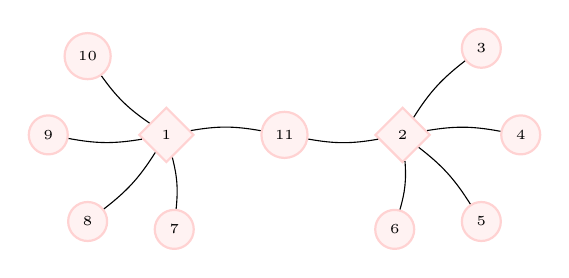
\begin{tikzpicture} 
\tikzset{vertex/.style = {circle,draw=pink!70,fill=pink!20,thick,minimum size=2mm}}
\tikzset{vert/.style = {diamond,draw=pink!70,fill=pink!20,thick,minimum size=2mm}}
% vertices
\node[vert] (1) at  (1.5,0) {{\tiny $2$}};
\node[vertex] (3) at  (2.5,1.1) {{\tiny $3$}};
\node[vertex] (4) at  (3,0) {{\tiny $4$}};
\node[vertex] (5) at  (2.5,-1.1) {{\tiny $5$}};
\node[vertex] (10) at  (1.4,-1.2) {{\tiny $6$}};
\node[vertex] (11) at  (-1.4,-1.2) {{\tiny $7$}};
\node[vert] (2) at (-1.5,0) {{\tiny $1$}};
\node[vertex] (6) at (-2.5,1) {{\tiny $10$}};
\node[vertex] (7) at (-2.5,-1.1) {{\tiny $8$}};
\node[vertex] (8) at (-3,0) {{\tiny $9$}};
\node[vertex] (9) at (0,0) {{\tiny $11$}};
%edges
\draw[-,=latex] (6) to[bend left=-10] (2);
\draw[-,=latex] (7) to[bend left=-10] (2);
\draw[-,=latex] (8) to[bend left=-10] (2);
\draw[-,=latex] (9) to[bend left=-10] (2);
\draw[-,=latex] (11) to[bend left=-10] (2);
\draw[-,=latex] (3) to[bend left=-10] (1);
\draw[-,=latex] (10) to[bend left=-10] (1);
\draw[-,=latex] (4) to[bend left=-10] (1);
\draw[-,=latex] (5) to[bend left=-10] (1);
\draw[-,=latex] (9) to[bend left=-10] (1);
%\draw[->,>=latex,dashed] (1) to[bend left] (9);
%\draw[->,>=latex,dashed] (2) to[bend left] (9);
%\draw[->,>=latex,dashed] (2) to[bend left] (6);
%\draw[->,>=latex,dashed] (2) to[bend left] (7);
%\draw[->,>=latex,dashed] (2) to[bend left] (8);
%\draw[->,>=latex,dashed] (1) to[bend left] (3);
%\draw[->,>=latex,dashed] (1) to[bend left] (4);
%\draw[->,>=latex,dashed] (1) to[bend left] (5);
\end{tikzpicture}
\end{center}
\caption{Network $G_{1}$, diamond shaped nodes correspond to individuals who choose to $express$.}
%%%%%%%%%%%
\label{connectorfigure}
%%%%%%%%%%%
\end{figure}
%
\begin{example} Consider the network $G_{1}$ in Figure \ref{connectorfigure}. Individuals $1$ and $2$ both have local popularity $\delta_1 = \delta_2 = 5 / \big( (1/5) (1+1 +1 +1 + 2) \big) = 25/6 >\delta^{*}$, therefore they play $express$ and $E = \{ 1,2\}$. While individuals $j \in \{ 3, \ldots,  9, 10 \}$ have a local popularity $\delta_j = 1/5 <\delta^{*}$ and individual $11$ has $\delta_{11}=4/10 <\delta^{*} $ , hence they play $hide$ and $C=\{ 3, \ldots, 10,11 \}$.
\end{example}

\bibliography{bib_thesis}
\bibliographystyle{plain}

\end{document}
%\footnotesize{  
%\bibliography{content/bib_thesis}{}
%\bibliographystyle{plain}}



